\chapter{Mecánica de Materiales}
\section{Introducción}

Supóngase a tarzán sujetándose de una liana, esa acción puede ser representada con un diagrama de cuerpo libre. Si Tarzán pesa 80Kg.
La tercera ley de Newton dice que: \emph{``toda acción corresponde a una reacción''}
\begin{equation}
    \sigma = \frac{P}{A}
\end{equation}
Pensando que la cuerda tiene una resistencia es de 28.48 MPa (Basándose de alguna fuente confiable), podemos encontrar la resistencia dividiendo:
\begin{equation*}
    \sigma = \frac{80kg}{0.554cm^2} = 144.4 \frac{kg}{cm^2}
\end{equation*}
Sin embargo, se debe usar un factor de seguridad para que las estructuras duren muchos más años, usando en éste caso el factor de 2, se divide dando $145.2 kg/cm^2$ cabe señalar que el factor de seguridad está dado por el material en defecto.
\subsection{Perfiles estructurales}
\subsubsection{Nomenclatura IMCA}
El Instituto Mexicano de la Construcción en Acero A.C. (IMCA) consideró conveniente
designar los perfiles de acero con sólo dos letras, una ideográfica y la otra, abreviatura de su
descripción, en lugar de las tres o más siglas tradicionales . En la figura 1 se indican las
equivalencias:
\begin{figure}[h!]
\centering
  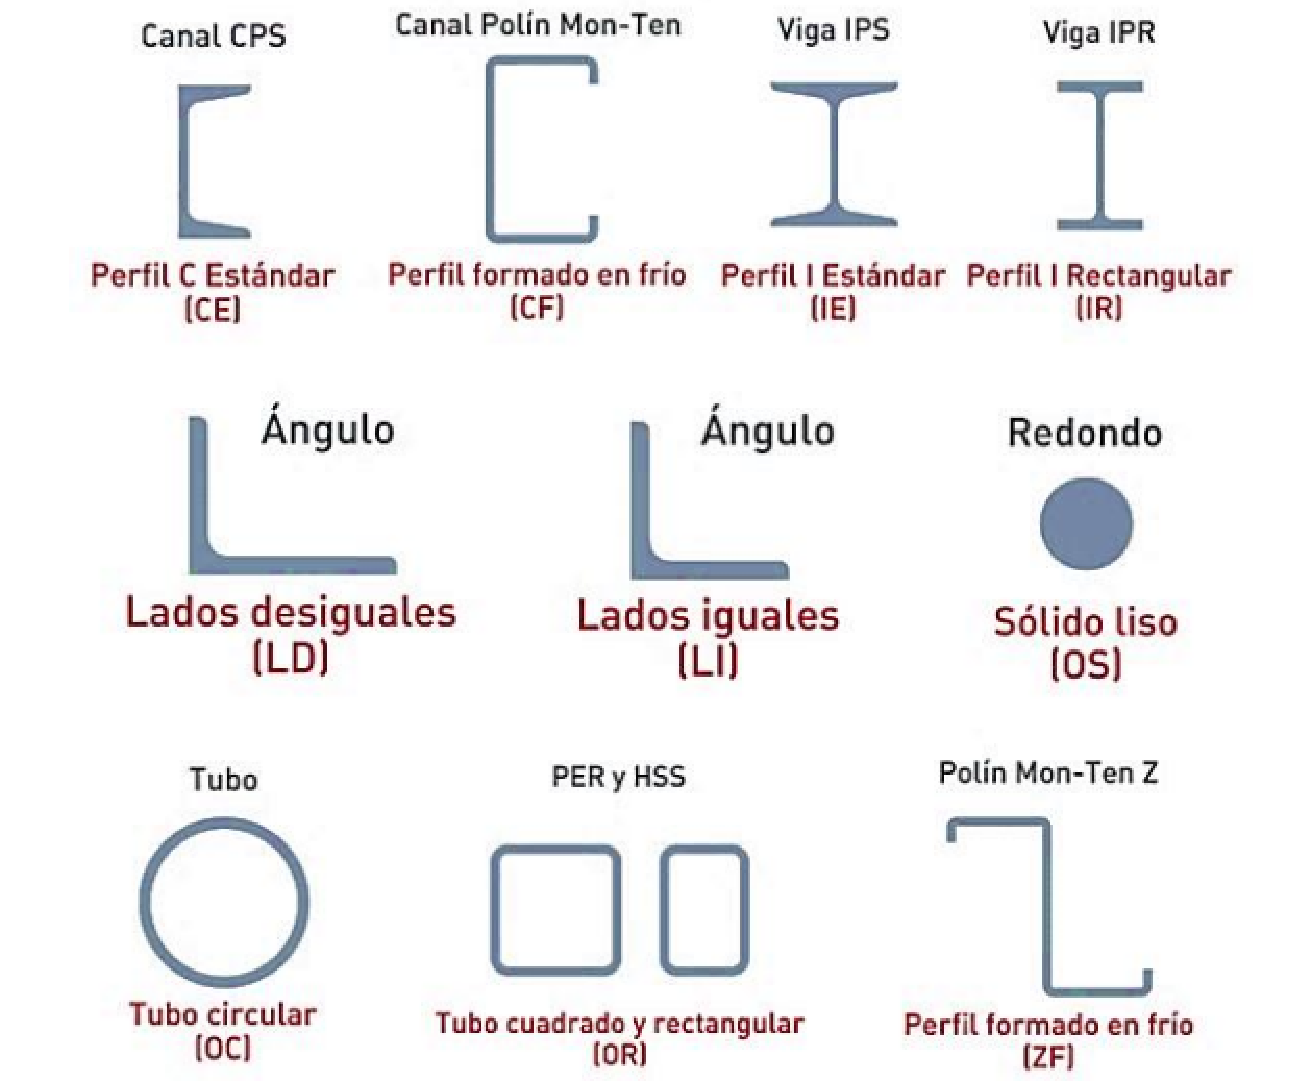
\includegraphics[width=0.5\textwidth]{mm6.pdf}
  \caption{Designación de perfiles de acero}
  \label{mm6}
\end{figure}

\subsubsection{ASTM A-36}

Esta norma es aplicable a una variedad de perfiles estructurales laminados en caliente y a placas de la misma calidad que están disponibles en el mercado mexicano. Tiene un esfuerzo de fluencia de $2530 kg/cm^2$ (250 MPa, 36 ksi), y su soldabilidad es adecuada. Se desarrolló desde hace muchos años en Estados Unidos para la fabricación de estructuras remachadas, atornilladas y soldadas, mejorando el contenido de carbono de los aceros disponibles en aquella época, como el ASTM A-7. Con la innovación de este tipo de acero, las conexiones soldadas empezaron a desplazar a las remachadas que pronto desaparecieron.

\subsubsection{ASTM A-29}

Se usa con mucha frecuencia en la construcción de edificios de acero, también es un grado de acero común en barras y perfiles (ángulos, canales de calidad estructural). El acero A529 básico incluye grado 50 para perfiles de los grupos 1 y 2 de la ASTM; placas hasta de una pulgada de grueso y 12 pulgadas de ancho (25x305 mm) y barras hasta de 2.5 pulg (64mm) de grueso. Las resistencias a la fluencia y máxima son de 42 y 60 ksi (2,950 y 4,220 a 5,975$kg/cm^2$)

\subsubsection{ASTM A-992}
El A-992 es la edición reciente (1998) de la lista de aceros estructurales en Estados Unidos. Se produjo para usarse en construcción de edificios, y está disponible solamente en perfiles tipo W (Vigas IPR, IMCA IR). Para propósitos críticos se trata de un esfuerzo de fluencia mínimo especificado de 354 MPa o 50 ksi (3,515 $kg/cm2$) La relación entre la resistencia a la fluencia y la resistencia máxima no es mayor de 0.85 y el carbono equivalente no excede de 0.50\%.Ofrecen características excelentes de soldabilidad y ductilidad.

\subsection{Ley de Hooke}
\begin{table}[h!]
  \centering
    \begin{tabular}{@{}cc@{}}
    \toprule
    Número & Kg      \\ \midrule
    1      & 1009    \\
    2      & 1010    \\
    3      & 1011    \\
    4      & 1014    \\
    5      & 1021    \\
    6      & 1023    \\
    7      & 1023    \\
    8      & 1034    \\
    9      & 1045    \\
    10     & 1048    \\
    Promedio:  & 1024.75 \\ \bottomrule
    \end{tabular}
    \caption{Aplicación del esfuerzo sobre un cuerpo}
    \label{tabmm1}
\end{table}

\begin{figure}[h!]
\centering
  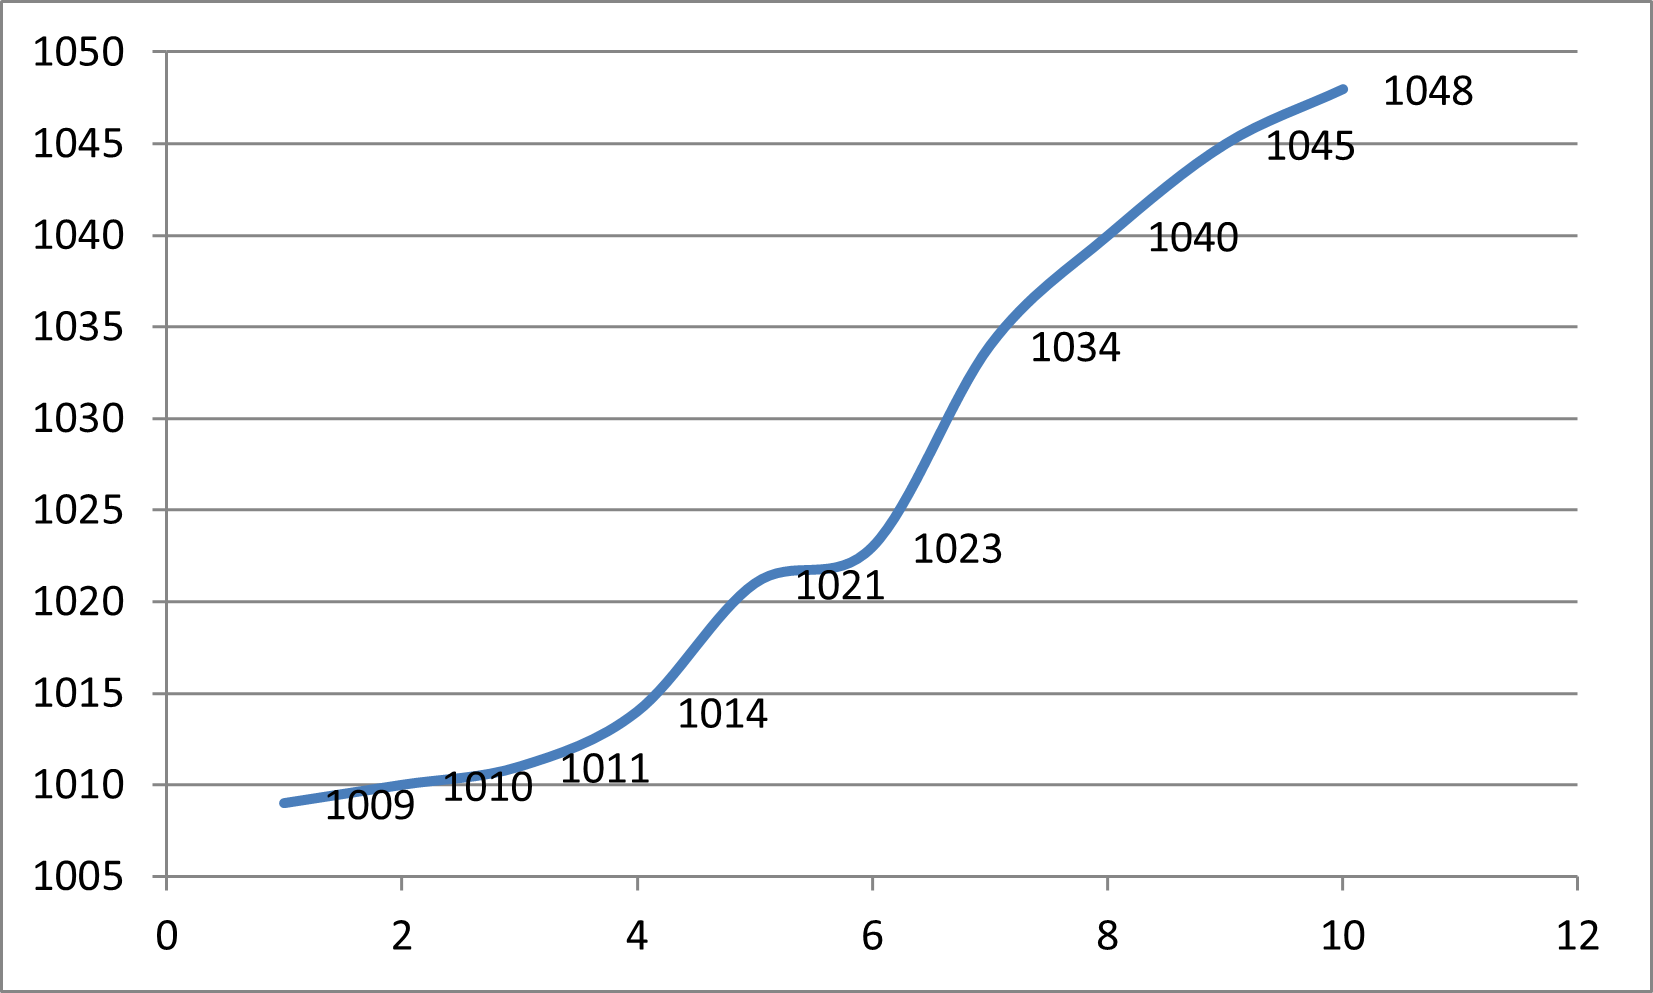
\includegraphics[width=0.5\textwidth]{mm1.png}
  \caption{Gráfica del esfuerzo sobre un cuerpo}
  \label{mm1}
\end{figure}

Los limites para el acero, son dados por una F.S. (factor de reducción de resistencia en el punto 0.6) la resistencia máxima debe de ser de $614.85 Kg/cm^2$
con éste dato, se plantea el siguiente problema:

\begin{problem}[Resorte]
    Calcular cuánto valen sus esfuerzos y desplazamientos de la figura \ref{mm2}
\end{problem}

\begin{figure}[h!]
\centering
  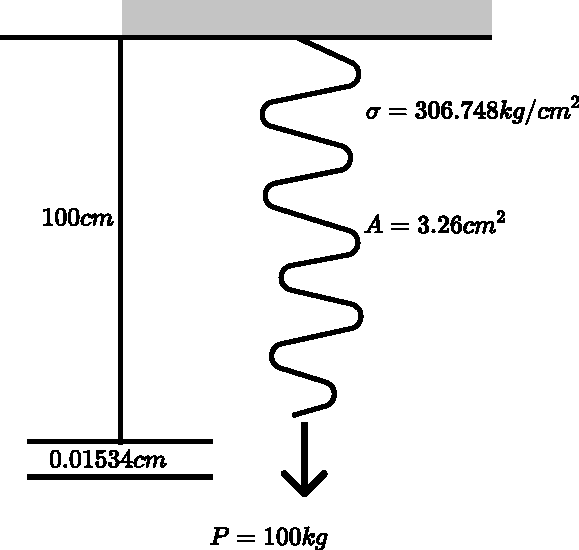
\includegraphics[width=0.5\textwidth]{mm2.pdf}
  \caption{Esquema del problema}
  \label{mm2}
\end{figure}

Se calcula el esfuerzo equivalente a:
\begin{equation*}
    \sigma = \frac{P}{A} = \frac{1000Kg}{3.26cm^2} = 306.748\frac{Kg}{cm^2}
\end{equation*}
Ese es el esfuerzo que produce una tonelada. Esto implica que es aceptable para el esfuerzo máximo.
\begin{figure}[h!]
\centering
  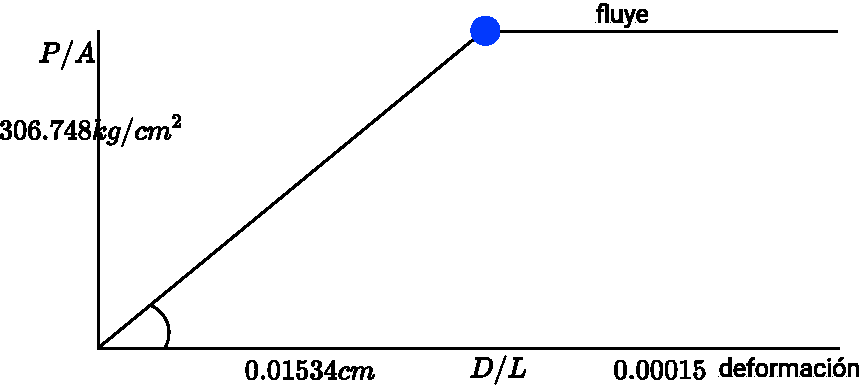
\includegraphics[width=0.5\textwidth]{mm3.pdf}
  \caption{Esfuerzos con deformaciones}
  \label{mm3}
\end{figure}

Ahora para calcular el desplazamiento, se tiene un triángulo rectángulo donde se tienen los valores de los catetos, así que aplicamos la siguiente fórmula:

\begin{equation}
    \tan{\alpha} =\frac{\sigma}{\epsilon}\implies \frac{\frac{P}{A}}{\frac{D}{L}} = \frac{PL}{EA} 
\end{equation}
Sustituyendo el esfuerzo experimentado:
\begin{equation*}
    E = 2 \times 10^{6}\frac{Kg}{cm^2} = 0.01534cm
\end{equation*}
Al tener una carga más grande, se necesitaría un mayor esfuerzo, pero hay un límite cuando el material empieza a fluir para romperse.
Si la fuerza es de tensión, entonces el elemento se alarga y si es de compresión se va a disminuir.

\begin{problem}[Colocando dos apoyos, se pone una cuerda con una cierta longitud]
    Pasando del punto a al punto b, podemos desplazarnos sólo con las manos.
\end{problem}

\begin{figure}[h!]
\centering
  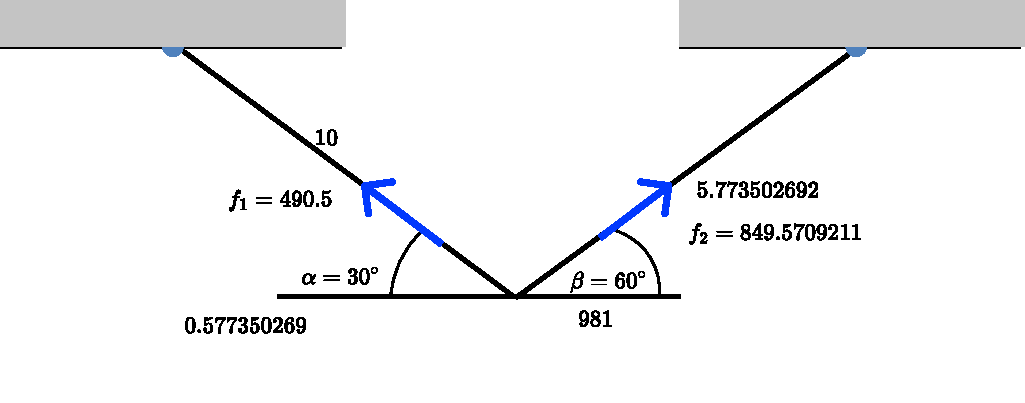
\includegraphics[width=0.5\textwidth]{mm4.pdf}
  \caption{Hombre colgado de una cuerda}
  \label{mm4}
\end{figure}

Se va a comprobar que la longitud de la cuerda es correcta, supóngase que del punto de apoyo al punto b vale 10m,la otra parte al sufrir una expansión, aumenta 0.1m así que sumando ambas partes nos da un total de 10.1m.
Si la carga es de 80kg, se necesita calcular la fuerza en el cable, las dos fuerzas van hacia arriba (Proyección coseno, cateto adyacente), obteniendo las constantes cuando colocamos el punto exactamente en la mitad (5.05m):
\begin{align*}
    \sin{\alpha} = 0.140 & ca = 0.990&&\sin{\beta} = 0.140&& cb = 0.990
\end{align*}
se logra una matriz:
\begin{align*}
    &0.990&&0.990\\
    &0.140&&0.140
\end{align*}
Invirtiendo la matriz:
\begin{align*}
    &-0.505&&3.561&&F_1= 284.9955N\\
    &0.505&&3.561&&F_{2} = 284.9955N
\end{align*}

Tabulando las fuerzas a diferentes condiciones:
\begin{table}[h!]
  \centering
    \begin{tabular}{@{}cccc@{}}
    \toprule
        & D &        & DES(m) \\ \midrule
    F1= & 0 & 80     & 0.100  \\
    F1= & 1 & 181.30 & 0.433  \\
    F1= & 2 & 233.42 & 0.570  \\
    F1= & 3 & 264.11 & 0.651  \\
    F1= & 4 & 280.46 & 0.695  \\
    F1= & 5 & 284.96 & 0.709  \\ \bottomrule
    \end{tabular}
    \caption{Tabulación de las fuerzas}
    \label{tabmm2}
\end{table}

\begin{figure}[h!]
\centering
  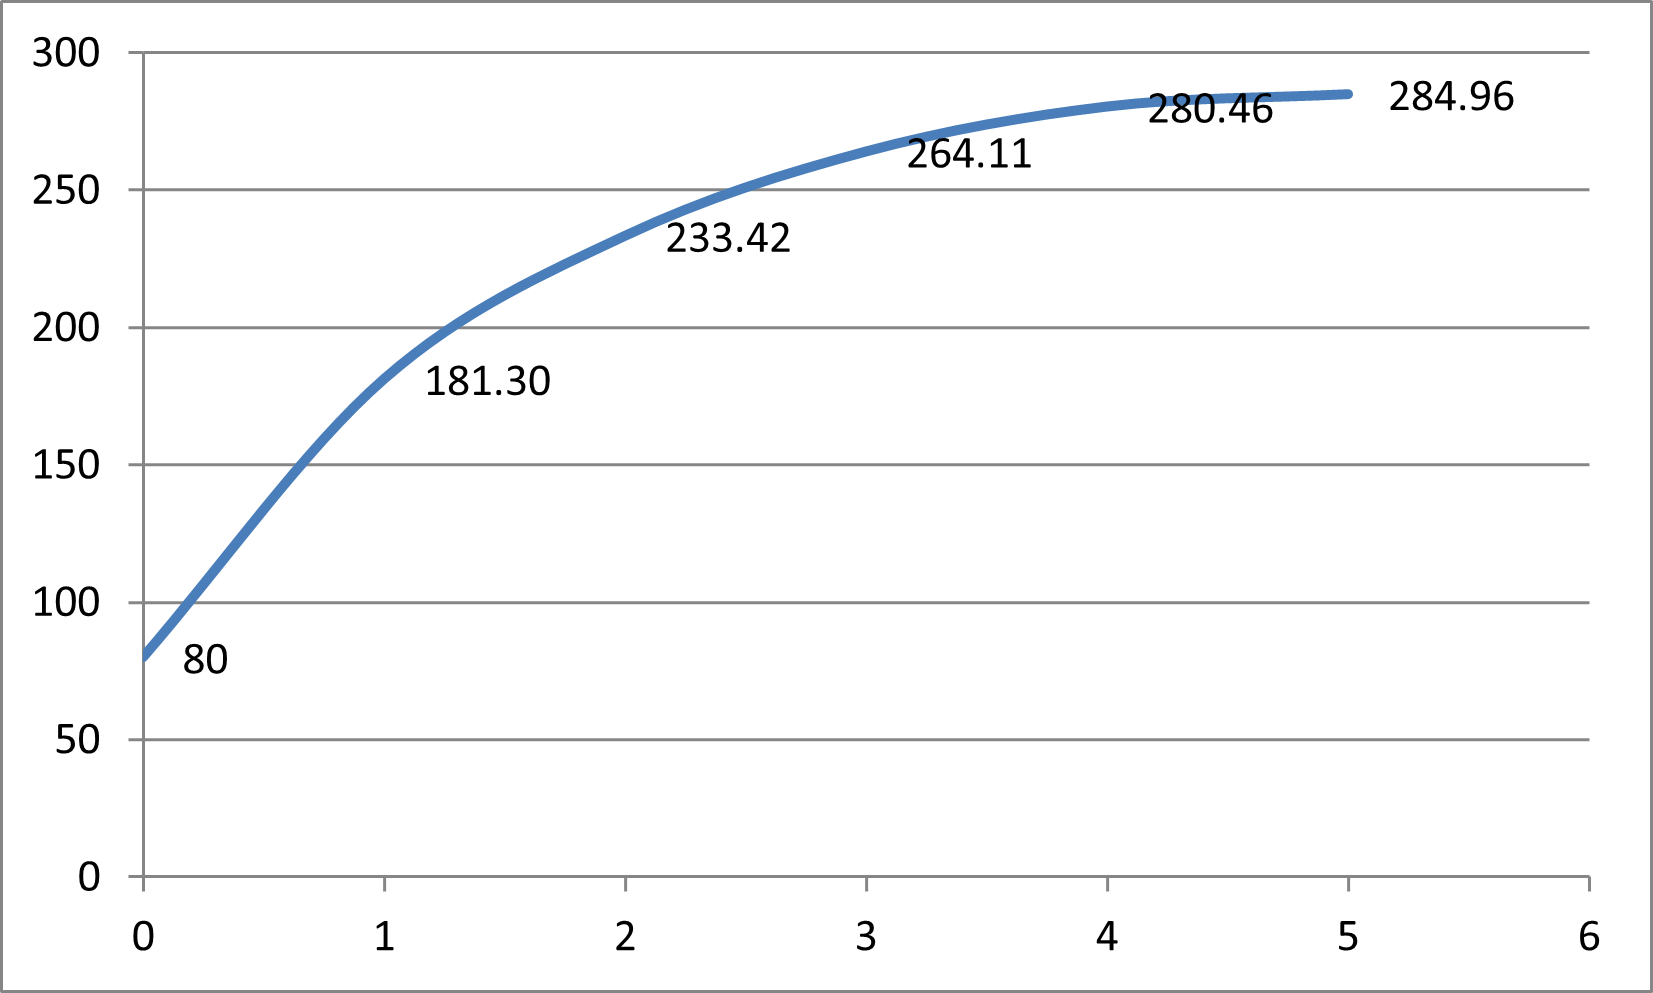
\includegraphics[width=0.5\textwidth]{mm5.png}
  \caption{Gráfica de las fuerzas}
  \label{mm5}
\end{figure}

Se propone resolver un problema con cinco barras y una fuerza que actúa en el nodo cuatro del eje x, yendo hacia la izquierda.
Se propone que los signos sean positivos hacia la derecha, como se muestra en la figura \ref{mm7}, ahora se pretende resolver el equilibrio externo, en la figura \ref{mm8}


\begin{figure}[h!]
\centering
  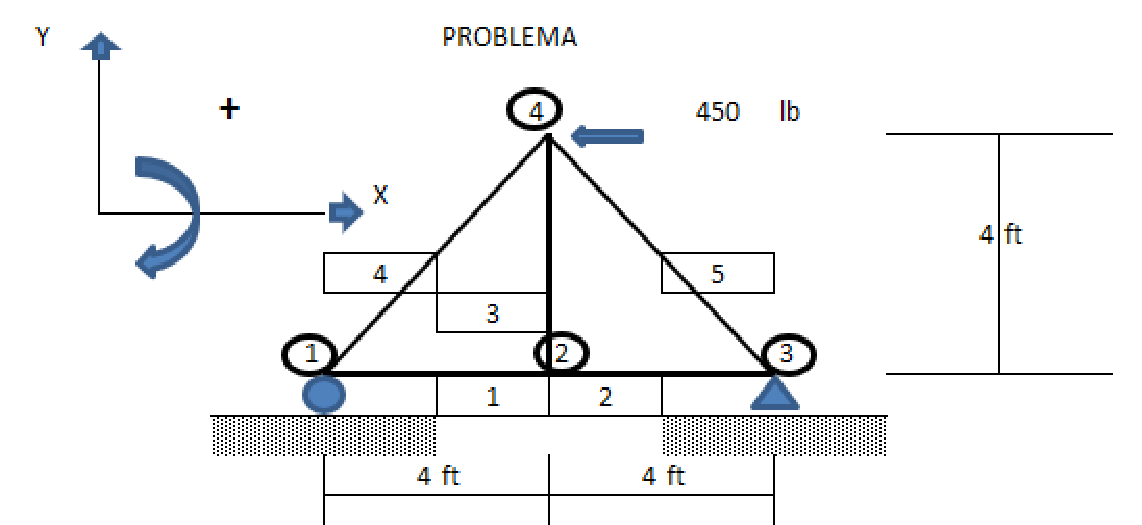
\includegraphics[width=0.5\textwidth]{mm7.pdf}
  \caption{Esquema del problema}
  \label{mm7}
\end{figure}

Se necesita estática, es decir que la suma de las fuerzas sea cero, para que haya equilibrio, en el nodo 3 se necesita la fuerza de 450lb para contrarrestar el nodo 4. Sabiendo que el momento es fuerza por distancia, podemos hacer suma de momentos (Igual a cero en cualquier punto).
Así que $Ry_3=F\cdot d=\frac{450lb\cdot 4ft}{4ft+4ft}=225lb$, al no haber fuerza externa vertical, tiene que estar equilibrada en algún momento de la reacción del nodo 1, debe ser 225lb también.

\begin{figure}[h!]
\centering
  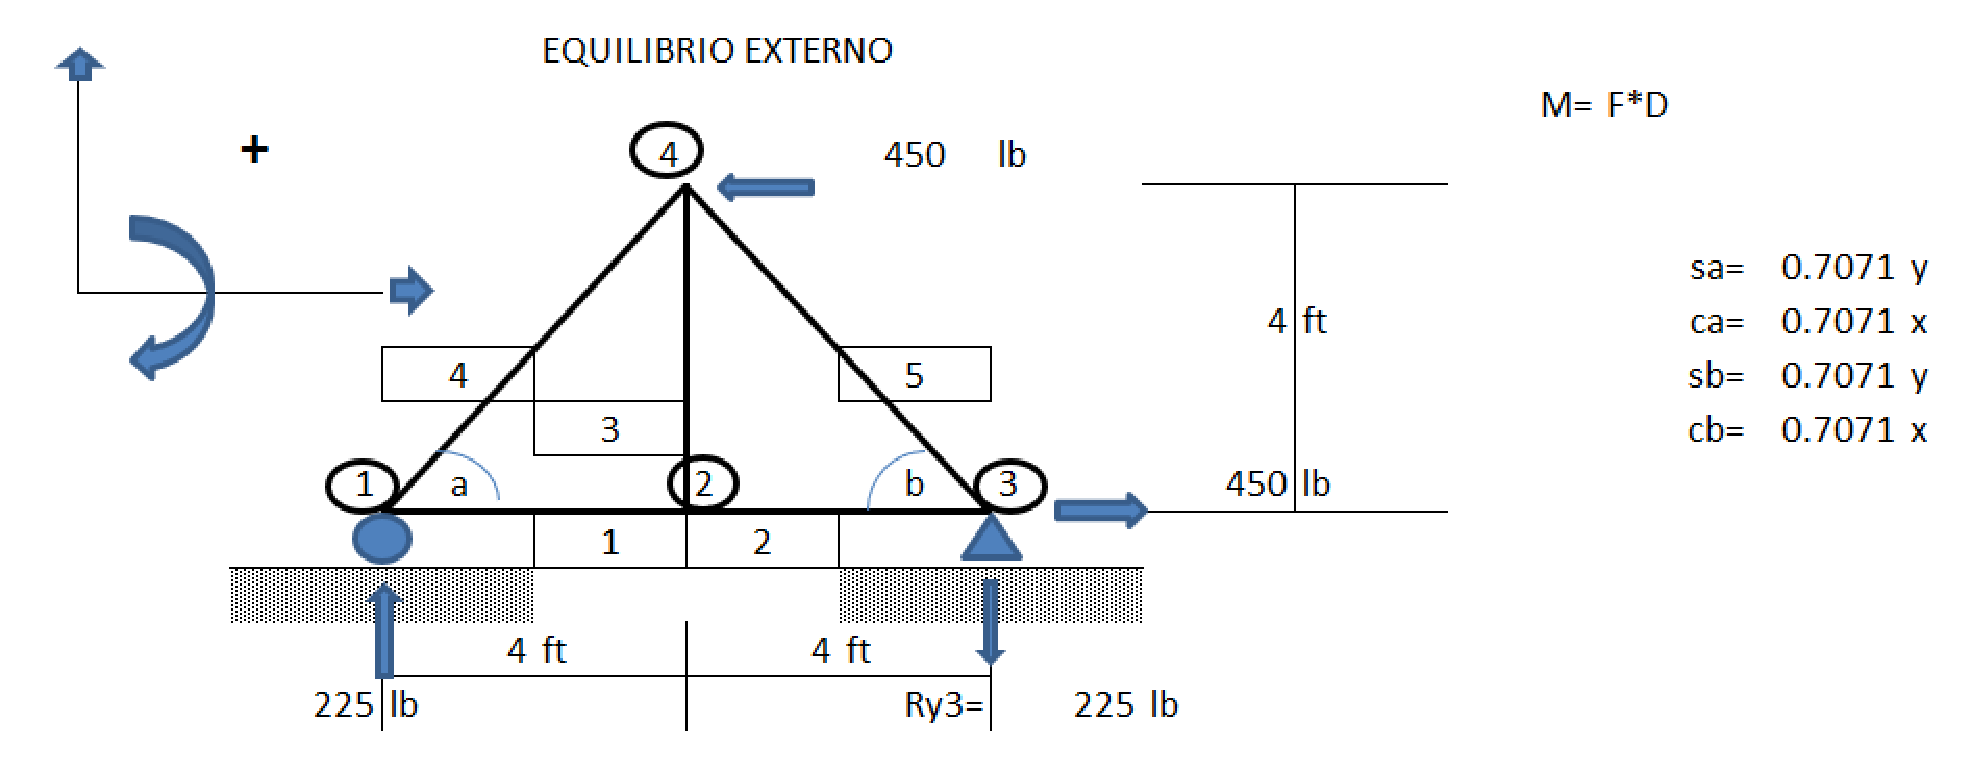
\includegraphics[width=0.5\textwidth]{mm8.pdf}
  \caption{Equilibrio externo}
  \label{mm8}
\end{figure}

\begin{figure}[h!]
\centering
  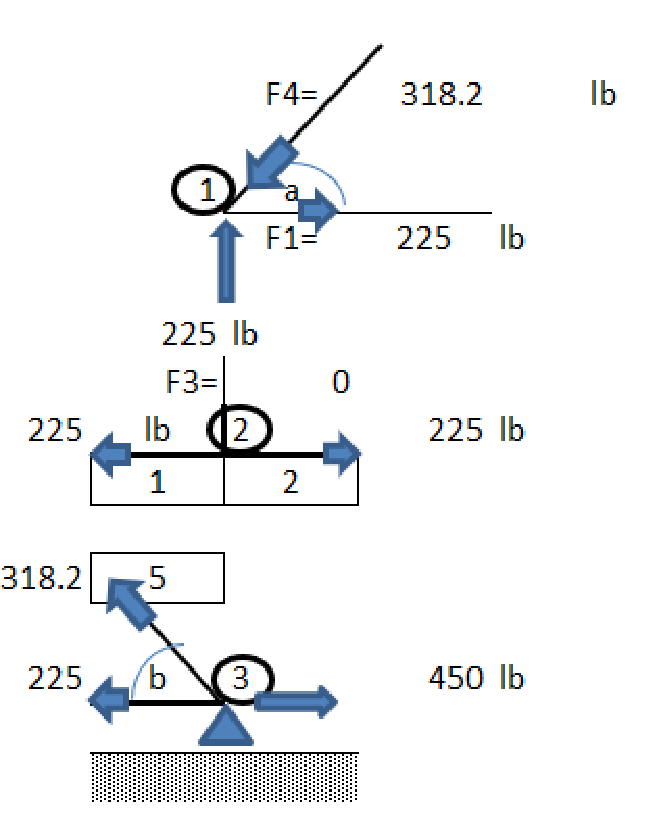
\includegraphics[width=0.5\textwidth]{mm10.pdf}
  \caption{Diagrama de cuerpo libre}
  \label{mm10}
\end{figure}
\begin{example}
  Se pretende encontrar cuántas fuerzas puede tener éste problema de la figura \ref{mm11}
\end{example}

\begin{figure}[h!]
\centering
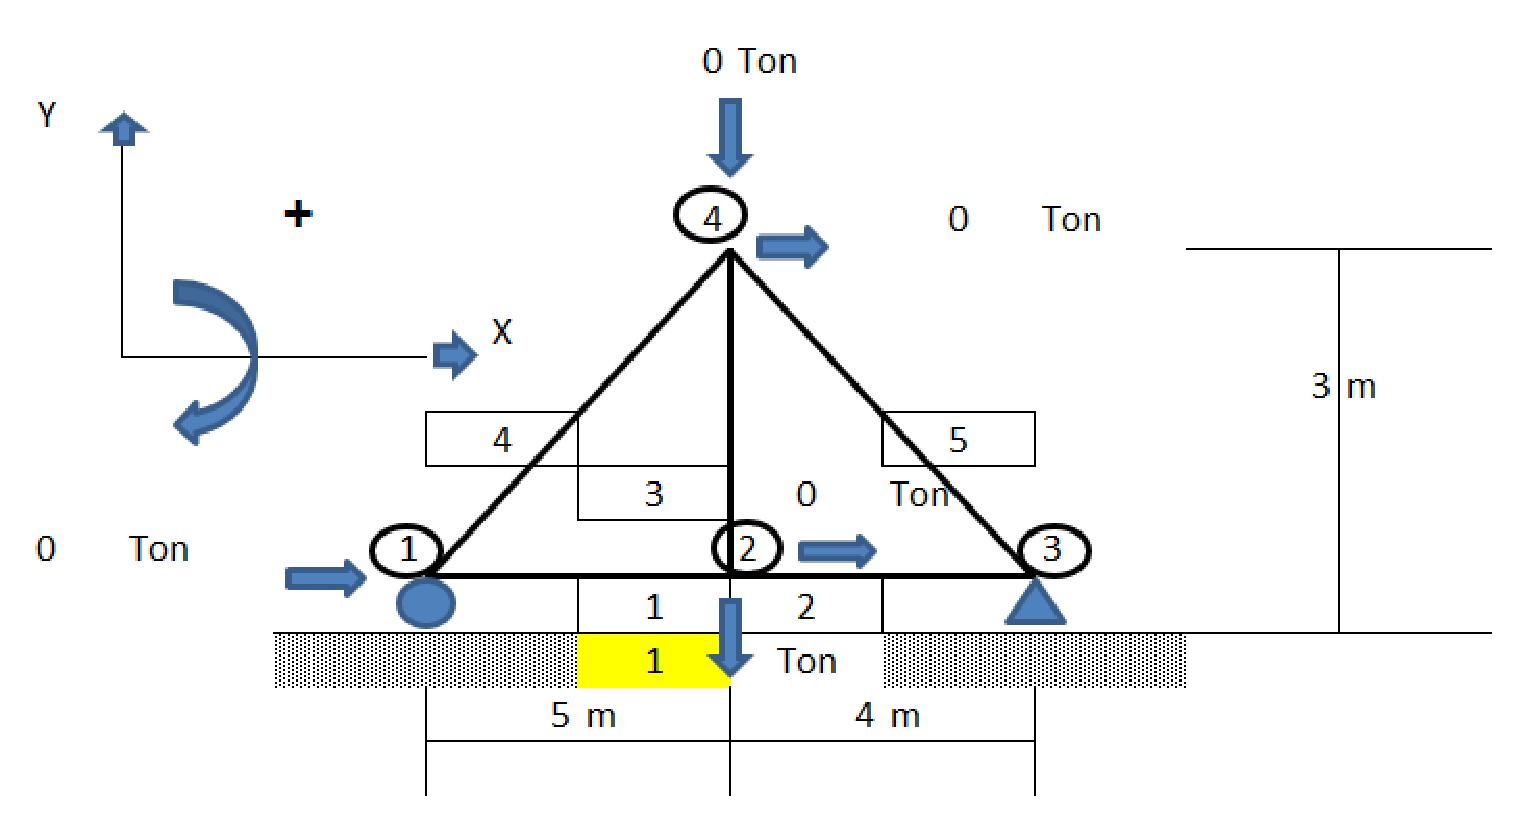
\includegraphics[width=0.5\textwidth]{mm11.pdf}
\caption{Esquema del problema}
\label{mm11}
\end{figure}
\textit{ Sol. }

Se buscan los nudos libres, semilibres y no libres (Cómo el 3), como se puede observar actúan dos fuerzas en los nudos 2 y 4, mientras que sólo actúa una fuerza en el nudo 1,
en total cinco fuerzas externas están actuando y tres incógnitas al equilibrio externo.

Para calcular el equilibrio externo, se aplica la tercera ley de newton:

\begin{figure}[h!]
\centering
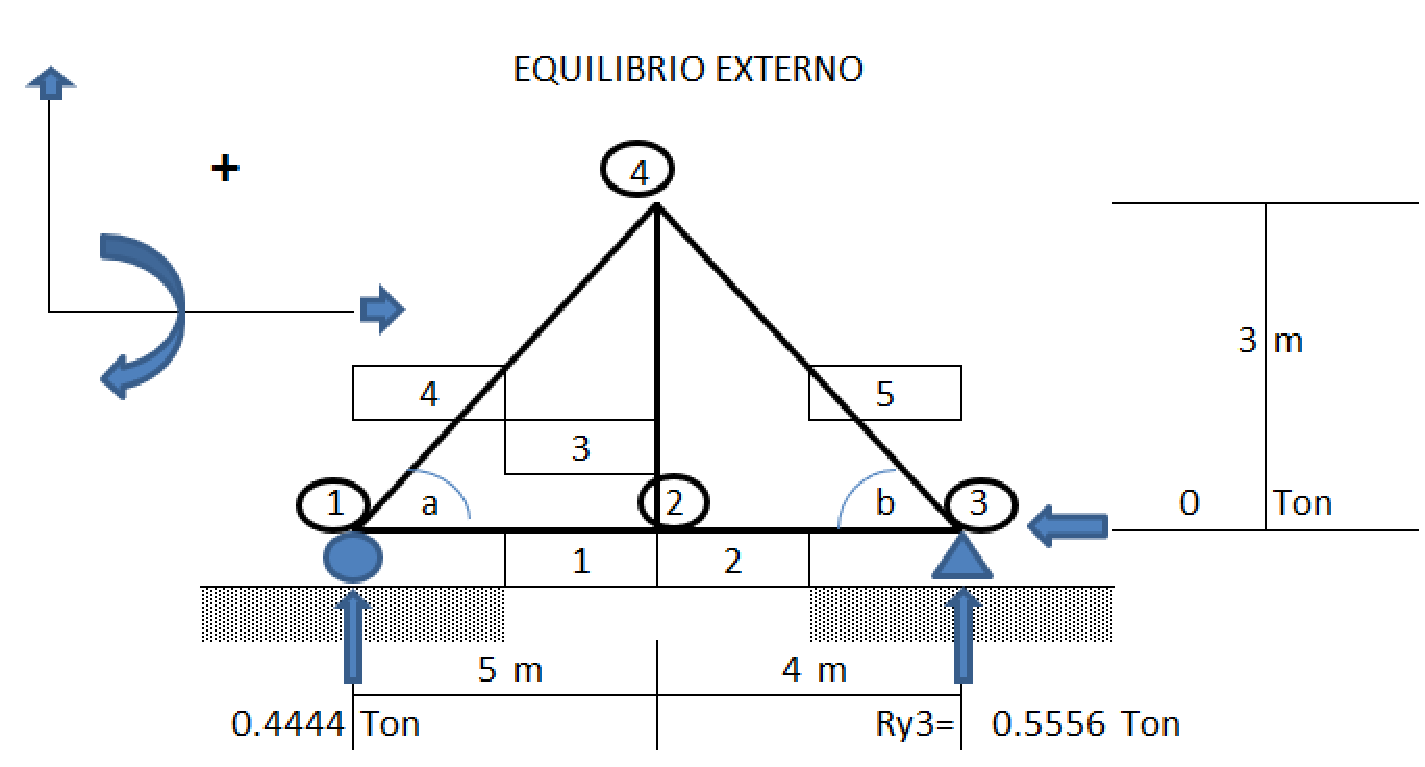
\includegraphics[width=0.5\textwidth]{mm12.pdf}
\caption{Equilibrio externo}
\label{mm12}
\end{figure}

Nótese que en la figura \ref{mm12}, la convención de signos cambia para dejar las fuerzas positivas. Calculando las distancias, se llega a:
\begin{align*}
  &sa = 0.5145y&&ca=0.8578x&&sb =0.6y&&cb= 0.8x
\end{align*}
Se procede a calcular las fuerzas internas en la figura \ref{mm13}:
\begin{figure}[h!]
\centering
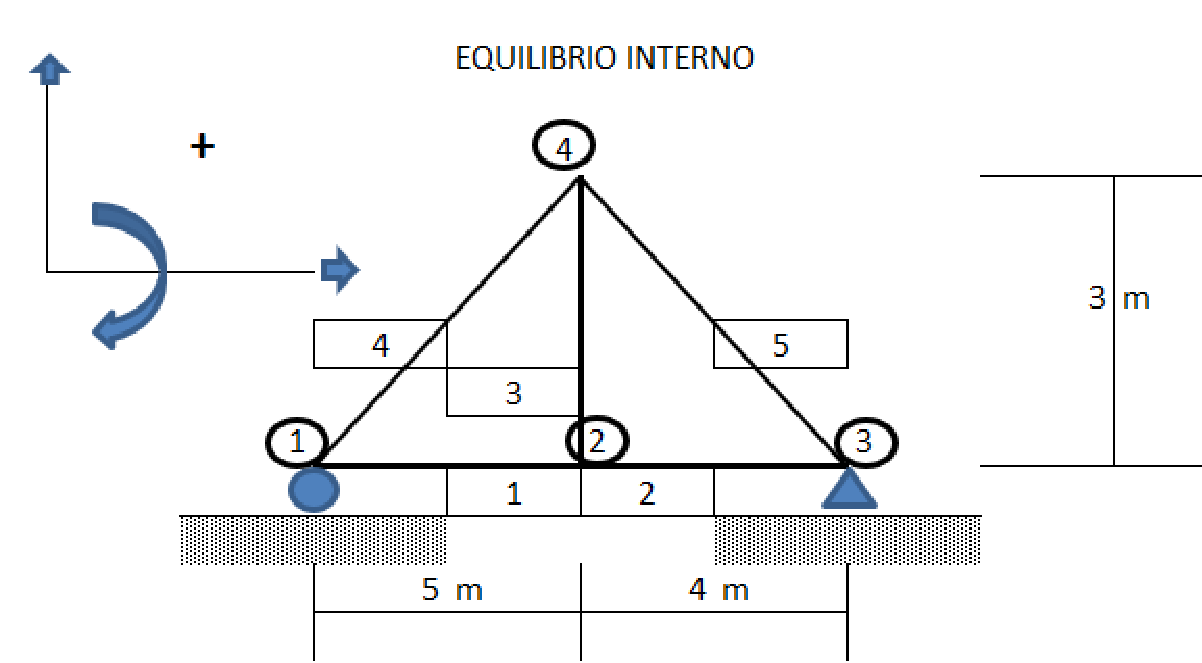
\includegraphics[width=0.5\textwidth]{mm13.pdf}
\caption{Equilibrio interno}
\label{mm13}
\end{figure}

Como la suma de las fuerzas debe de resultar cero, se encuentran las siguientes fuerzas:
\begin{align*}
  &F_1 =12.815ton&&F_2 = 1.8148ton&&F_3 = 21ton && F_4 = -28.939 ton&&F_5 =43.519\\
  &L_1 = 5m&&L_2 = 4m&&L_3 = 3m&&L_4 = 5.831m&&L_5 = 5m 
\end{align*}
El esquema para encontrar las fuerzas y longitudes de las barras, véase el esquema \ref{mm14}:

\begin{figure}[h!]
\centering
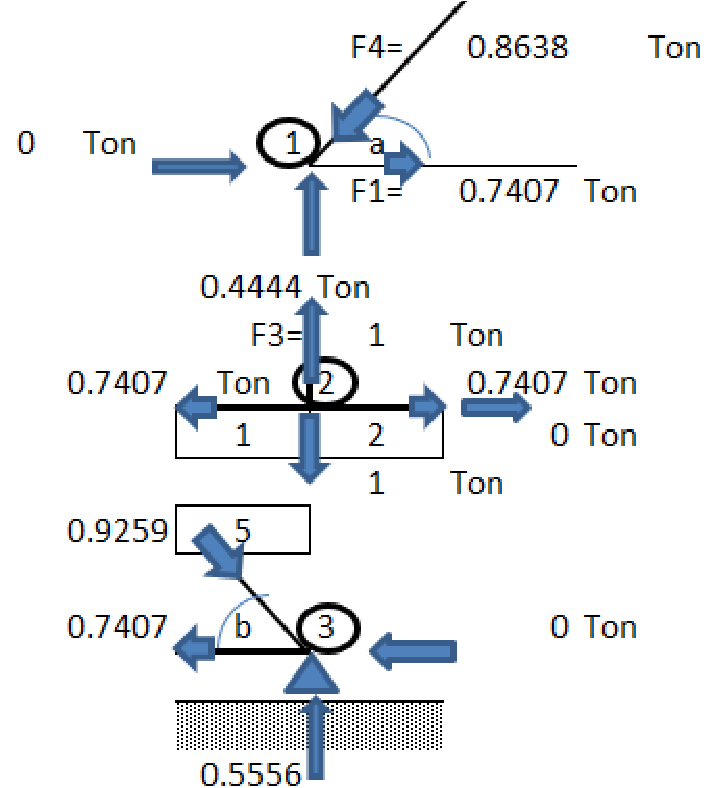
\includegraphics[width=0.5\textwidth]{mm14.pdf}
\caption{Cálculo de las fuerzas y longitudes}
\label{mm14}
\end{figure}

La fórmula para calcular los desplazamientos está dada por la ecuación \eqref{eqdesplazamientos}
\begin{equation}
  D =\sum \frac{PL}{EA} p
  \label{eqdesplazamientos}
\end{equation}

$D=$ desplazamiento, $P=$ fuerza interna en cada barra, $L=$ longitud de cada elemento, $E=$ módulo de elasticidad de el material ($2kg/cm^2$) para acero, $A=$ área de las barras y $p=$ Fuerza unitaria en donde $Y$ con el sentido que queremos el desplazamiento.

\begin{table}[h!]
  \centering
  \begin{tabular}{lllll}
                   & $P$        & $L$    & $p$             &                      \\
  1                & 12.8148    & 5      & 0.7407          & 47.4622              \\
  2                & 1.8148     & 4      & 0.7407          & 5.3772               \\
  3                & 21         & 3      & 1               & 63                   \\
  4                & -28.9387   & 5.8309 & -0.8638         & 145.7657             \\
  5                & -43.5185   & 5      & -0.9259         & 201.4746             \\
                   &            &        &                 & 463.0799             \\
  $T/m^2$          & $m^2$      &        & $D=\frac{E}{A}$ & $8.08\times 10^{-3}$ \\
  $E=2\times 10^7$ & $A=0.0028$ &        &                 &                     
  \end{tabular}
  \caption{Resultados}
  \label{tabmm3}
\end{table}
%%%%%%%%%%%%%%%%
%%%%%%%%%%%%%%%%
%%%%%%%%%%%%%%%%
%%%%%%%%%%%%%%%%
%%%%%%%%%%%%%%%%
%%%%%%%%%%%%%%%%
%%%%%%%%%%%%%%%%
%%%%%%%%%%%%%%%%
%%%%%%%%%%%%%%%%
%%%%%%%%%%%%%%%%
%%%%%%%%%%%%%%%%
%%%%%%%%%%%%%%%%
%%%%%%%%%%%%%%%%
\begin{example}
  Diseñe la siguiente armadura (Figura \ref{mm15}), con acero a 36 y calcule el área y el desplazamiento vertical en el nudo 1.
\end{example}
\begin{figure}[h!]
\centering
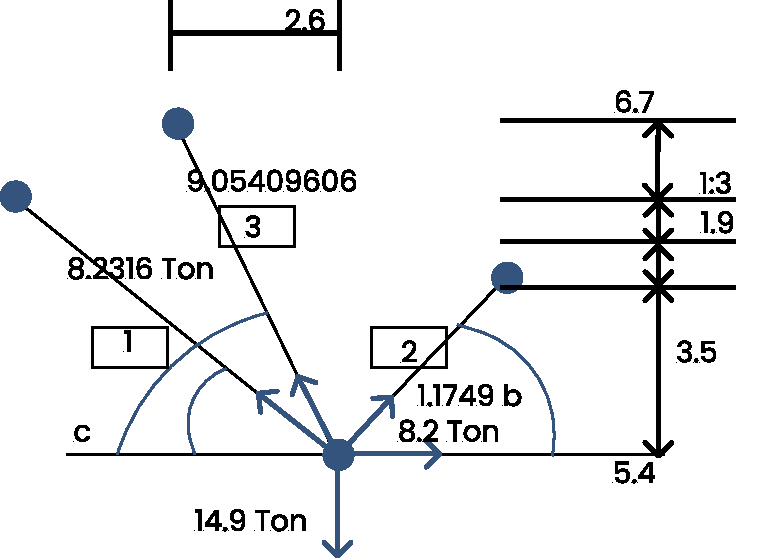
\includegraphics[width=0.5\textwidth]{mm15.pdf}
\caption{Armadura con acero a 26}
\label{mm15}
\end{figure}
\textit{ Sol. }

Se debe definir que las cargas deben estar en toneladas, las distancias en metros, no hay que perder de vista el signo de las fuerzas.
Se sabe que la proyección de la barra uno con la barra dos, debe ser igual a 8 y la proyección en y de ambas fuerzas deben dar 14.7 Ton,
Las longitudes de las barras se encuentran a partir de las proyecciones, primero se obtiene el $\sin{(\alpha)=0.6862}$, $\cos{\alpha}=0.7274$, $\sin{(\beta)}=0.6268$ y $\cos{\beta}=0.7792$

\begin{table}[h!]
  \centering
  \begin{tabular}{@{}ccccc@{}}
  \toprule
    & L     & Po     & P     &           \\ \midrule
  1 & 7.286 & 16.625 & 0.787 & 95.282    \\
  2 & 5.903 & 5.252  & 0.734 & 22.767    \\
    &       &        & PLp=  & 118.04895 \\ \bottomrule
  \end{tabular}
  \caption{Proyecciones de las barras uno y dos.}
  \label{tabmm15}
\end{table}
Se plantea una ecuación en x,y que tiene que ver con las proyecciones:
\begin{align*}
  &x,y&& F_1&&F_2&&\\
  &- 0.7274&&0.7792&&- 8\\
  &0.6862&&0.6268&&145.7
\end{align*}
Se calcula la inversa:
\begin{align*}
  &- 0.6326981&&0.7865977&- 8&16.624571\\
  &0.6927234&&0.7342868&&14.7&&5.2522289
\end{align*}
Concluyéndose que la fuerza mayor es de 16.62
para saber cuánta área se necesita, pues está en función
de la raíz cuadrada del área propuesta.

Para calcular los desplazamientos, se debe comprobar el equilibrio, como en el diagrama: 
\begin{figure}[h!]
\centering
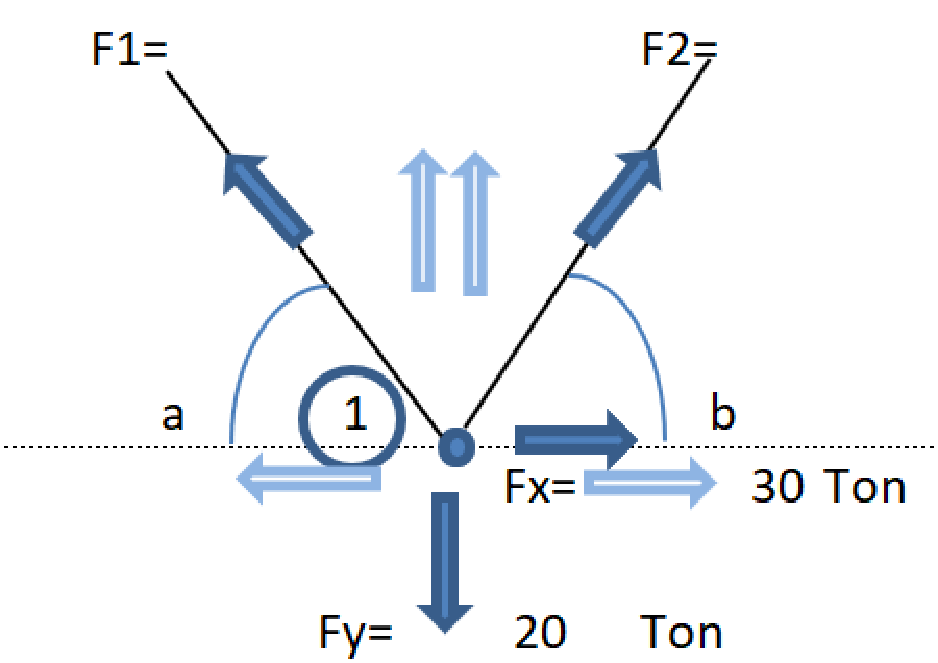
\includegraphics[width=0.5\textwidth]{mm16.pdf}
\caption{Equilibrio de la armadura}
\label{mm16}
\end{figure}

Cuando se proyecta la fuerza de 5, se proyectó 4.09 y la de 14.7 proyectó 12.09.
La suma de fuerzas debe dar cero. Teniendo el área, se utiliza una fórmula para el desplazamiento:
\begin{equation}
  D = \frac{P\cdot L}{E\cdot A}p
\end{equation}
Se tiene que resolver la carga real ($P$) y la carga unitaria ($p$),
pues ya se cuenta con el módulo de elasticidad (196), y el área propuesta,
de manera que $E\cdot A= 21903.256$ pues el cuadrado es de $0.3,\times 0.3m$, lo que de denota como $PLp$ de la tabla \ref{tabmm15}
con esos valores el desplazamiento da 0.00538956m, osea 5.38mm.%%%%%%%%%%%%%%%%
%%%%%%%%%%%%%%%%
%%%%%%%%%%%%%%%%
%%%%%%%%%%%%%%%%
%%%%%%%%%%%%%%%%
%%%%%%%%%%%%%%%%
%%%%%%%%%%%%%%%%
%%%%%%%%%%%%%%%%
%%%%%%%%%%%%%%%%
%%%%%%%%%%%%%%%%
%%%%%%%%%%%%%%%%
%%%%%%%%%%%%%%%%
%%%%%%%%%%%%%%%%
\begin{problem}[Resolver la siguiente armadura]
  \begin{figure}[h!]
  \centering
    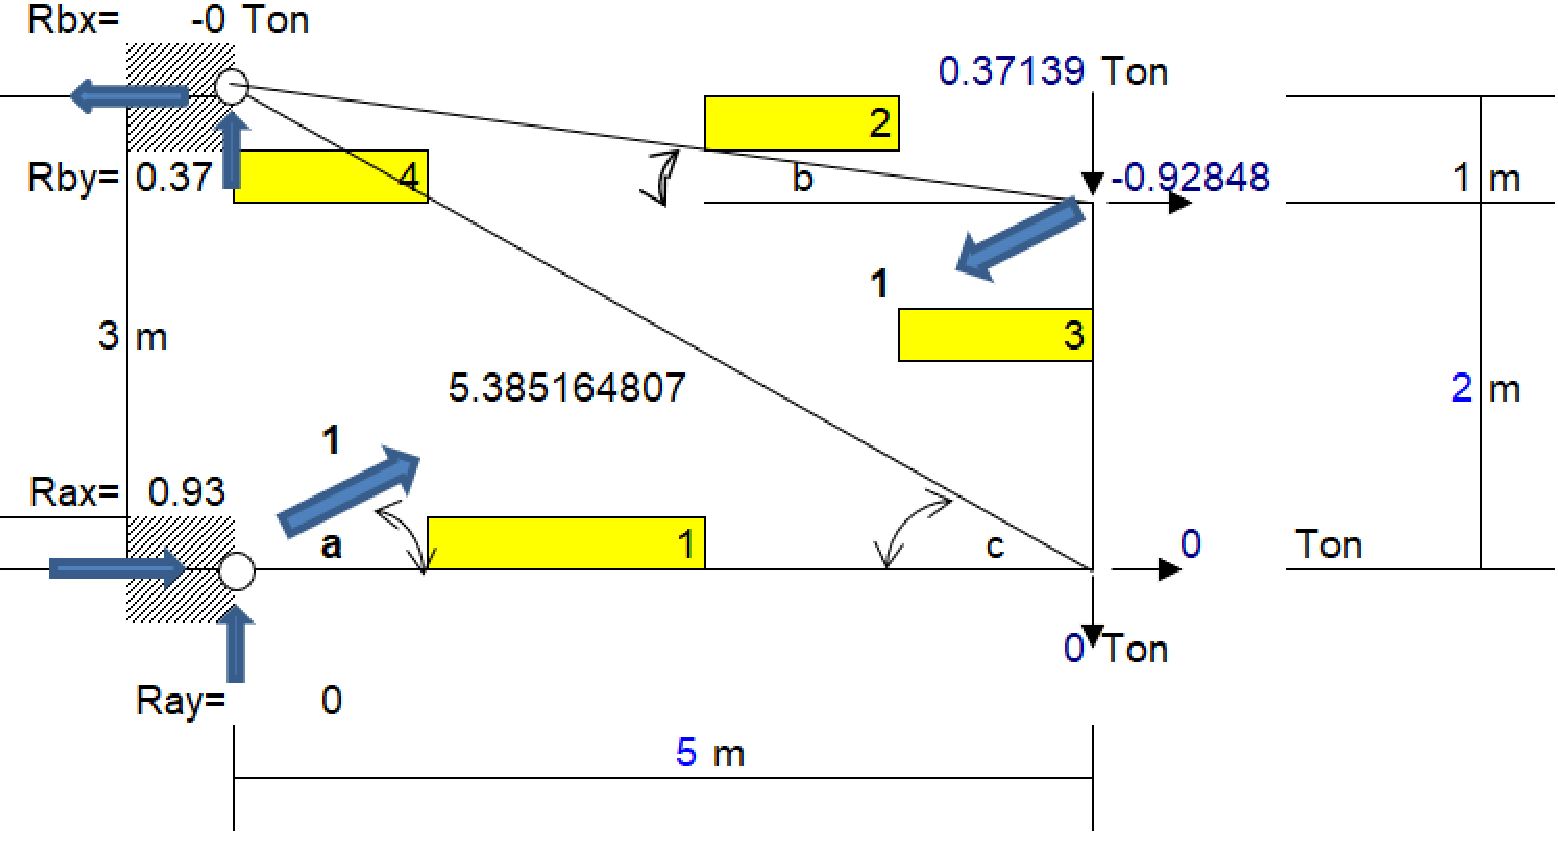
\includegraphics[width=0.5\textwidth]{mm17.pdf}
    \caption{Esquema del problema}
    \label{mm17}
  \end{figure}
\end{problem}

\textit{ Sol. }

  Se tienen cuatro barras, en cada nudo hay dos fuerzas, por ejemplo en el superior tiene 25 toneladas verticalmente y 25 toneladas horizontalmente; 
debajo hay otro nudo con 38 toneladas vertical y 45 toneladas horizontal; una longitud de 5m, una altura de 3m

Se debe calcular las longitudes, luego los ángulos (senos y cosenos), las fuerzas que entran y salen del nudo con respecto las barras para encontrar el equilibrio

\begin{align*}
  &\sin{\alpha} = 0.37139068&& \cos{\alpha} = 0.92847669\\
  &\sin{\beta} = 0.19611614&& \cos{\beta} = 0.98058068\\
  &\sin{\gamma} = 0.51449576&& \cos{\gamma} = 0.85749293\\
\end{align*}

\begin{table}[h!]
  \centering
  \begin{tabular}{@{}ccc@{}}
  \toprule
    & L/EA        & $P_0$    \\ \midrule
  1 & 5           & -48.3333 \\
  2 & 5.099020    & 35.69314 \\
  3 & 2           & -18      \\
  4 & 5.830951895 & 108.8444 \\
  5 & 5.385165    & 0        \\ \bottomrule
  \end{tabular}
  \caption{Distancias}
  \label{tabmm4}
\end{table}

La armadura es isostática porque tienen cuatro barras y cuatro nudos libres. Nótese sobre los desplazamientos.
Como hiperestática, se hará una nueva barra (5), de la figura \ref{mm18}
\begin{figure}[h!]
  \centering
\centering
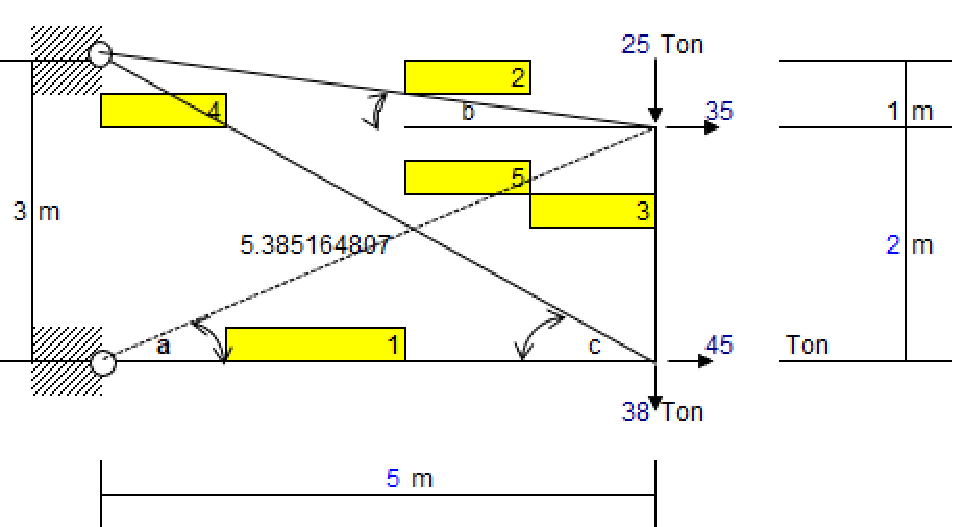
\includegraphics[width=0.5\textwidth]{mm18.pdf}
\caption{Hiperestática}
\label{mm18}
\end{figure}

El número de barras es mayor que el desplazamiento, por lo que es hiperestática, eso implica que hay una incógnita.
En lugar de la barra, se usa una fuerza unitaria pues se desconoce su valor, los resultados pueden contemplarse en la tabla \ref{tabmm4}.
Sabiendo que el desplazamiento es $Des=\frac{PL}{EA}\rho$,se procede a sustituir los valores obtenidos de la tabla \ref{tabmm5}

\begin{table}[h!]
  \centering
  \begin{tabular}{@{}ccccccc@{}}
  \toprule
    & $p$      & $\frac{L}{EA}$ & $P_0$    & $p^2\frac{L}{EA}$ & $p\cdot \frac{L}{EA}\cdot P(0)$ & $P$      \\ \midrule
  1 & -0.92848 & 5            & -48.3333 & 4.310345    & 224.3819                & -15.8806 \\
  2 & -0.94686 & 5.099020     & 35.69314 & 4.571535    & -172.329                & 68.78856 \\
  3 & -0.55709 & 2            & -18      & 0.62069     & 20.0551                 & 1.47164  \\
  4 & 1.082781 & 5.830951895  & 108.8444 & 6.836288    & 687.2047                & 70.99837 \\
  5 & 1        & 5.385165     & 0        & 5.385165    & 0                       & -34.9527 \\ \bottomrule
  \end{tabular}
  \caption{Obtención del desplazamiento}
  \label{tabmm5}
\end{table}

Resultando un desplazamiento de -33.0274m, así el diseño tendría:
\begin{align*}
  &f_y = 2560kg_/cm^2&& E = 20000000\\
  &f_{\max } = 1518kg_/cm^2&&EA = 93541.9904\\
  &A = 6.77099cm^2
\end{align*}

Plasmando éstos cálculos en la tabla \ref{tabmm6}
\begin{table}[h!]
  \centering
  \begin{tabular}{@{}cccccc@{}}
  \toprule
           &                                    & EA &             &            & L          \\ \midrule
  15.8806  & 15.8806006                         & 1  & -1.66666667 & 132.338339 & 5          \\
  68.78856 & 68.7885601                         & 1  & 0           & 0          & 5.09901951 \\
  1.47164  & 68.7885601                         & 1  & 0           & 0          & 2          \\
  70.99837 & 70.9983707                         & 1  & 1.94365063  & 804.648202 & 5.83095189 \\
  34.95266 & 70.9983707                         & 1  & 0           & 0          & 5.38516481 \\
           & PMax                               &    &             & 936.98654  &            \\ \bottomrule
  \end{tabular}
  \caption{Diseño de la armadura, donde el desplazamiento resulta 0.01001675m}
  \label{tabmm6}
\end{table}

Éste es un análisis para una estructura por el método de las flexibilidades. 
%%%%%%%%%%%%%%%%
%%%%%%%%%%%%%%%%
%%%%%%%%%%%%%%%%
%%%%%%%%%%%%%%%%
%%%%%%%%%%%%%%%%
%%%%%%%%%%%%%%%%
%%%%%%%%%%%%%%%%
%%%%%%%%%%%%%%%%
%%%%%%%%%%%%%%%%
%%%%%%%%%%%%%%%%
%%%%%%%%%%%%%%%%
%%%%%%%%%%%%%%%%
\subsection{Vigas}

Para comprenderlas se procede a realizar un problema introductorio (figura \ref{mm19})
\begin{example}
    Se tiene una viga con una carga perpendicular de 12 toneladas, empotrada con una longitud de 6m, en toda la viga las 8 toneladas se mantienen constantes (Fuerza negativa)
\end{example}
\begin{figure}[h!]
\centering
  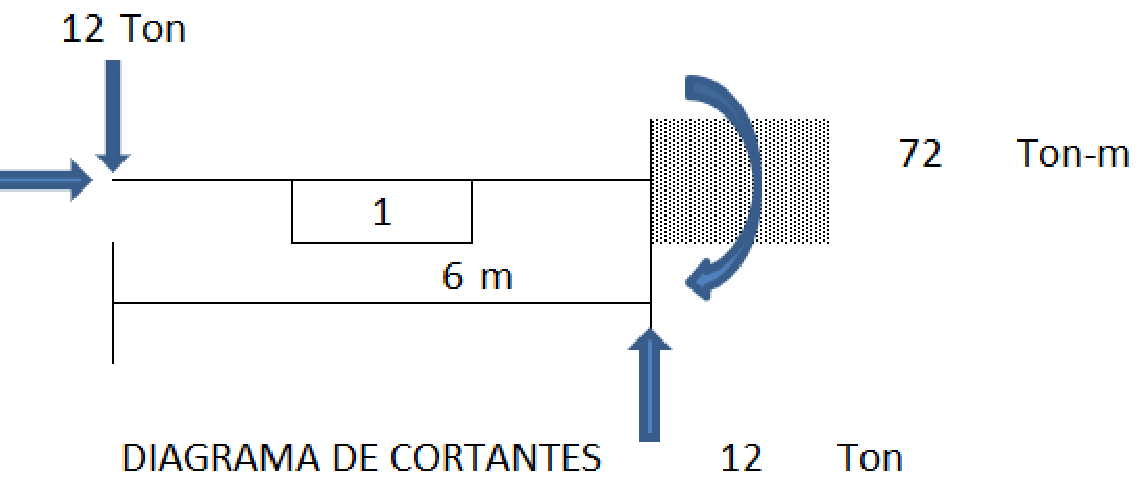
\includegraphics[width=0.5\textwidth]{mm19.pdf}
  \caption{Esquema del problema}
  \label{mm19}
\end{figure}
\textit{ Sol. }

Se tiene tomará el sentido perpendicular la fuerza negativa y se proyecta como en la figura \ref{mm20}

La integral en el problema, se puede ver que en el diagrama de cortantes se forma un triángulo, esta integral de las cargas es una constante,
(el área del rectángulo) es el diagrama de momentos de la figura \ref{mm21}
\begin{figure}[h!]
\centering
  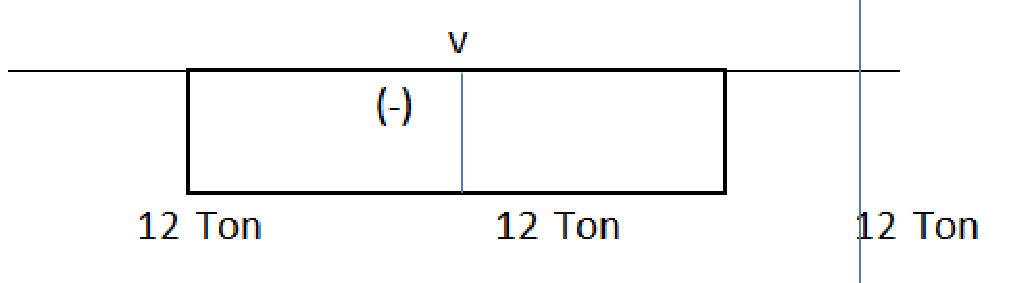
\includegraphics[width=0.5\textwidth]{mm20.pdf}
  \caption{Diagrama de cortantes}
  \label{mm20}
\end{figure}

\begin{figure}[h!]
\centering
  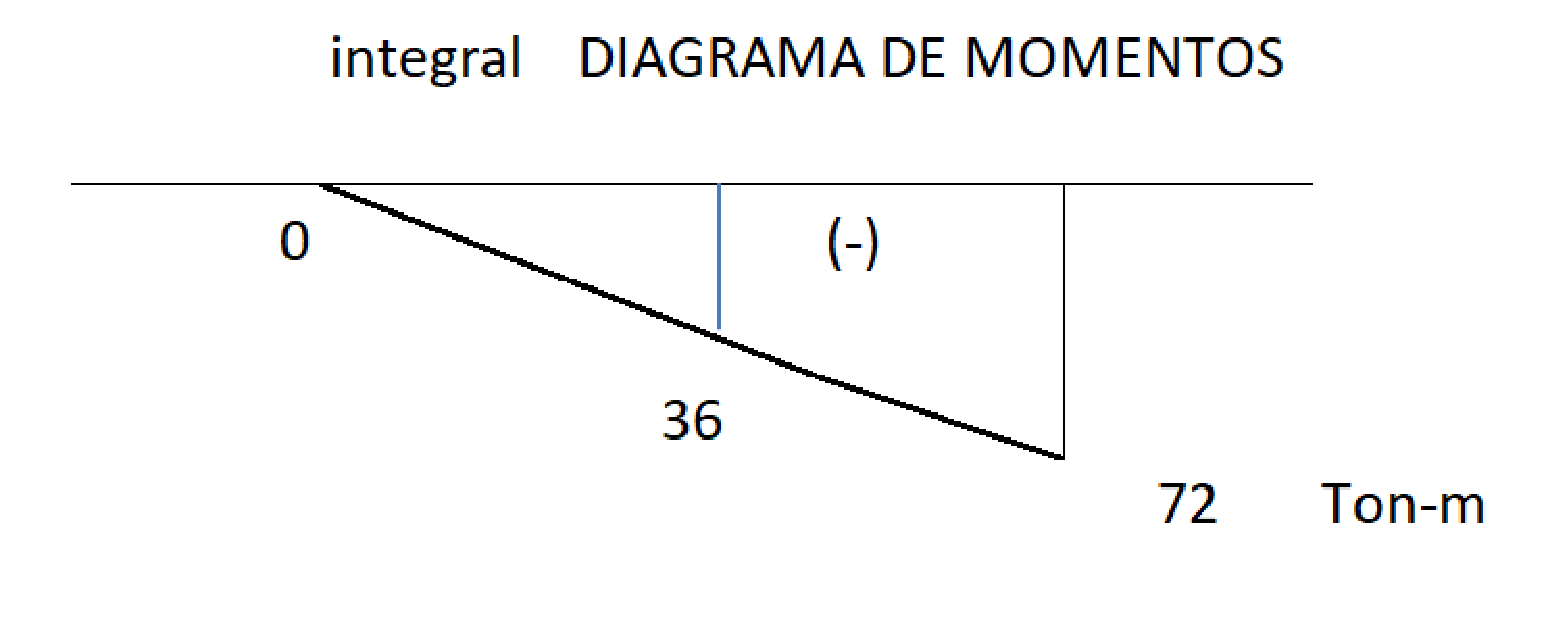
\includegraphics[width=0.5\textwidth]{mm21.pdf}
  \caption{Diagrama de momentos}
  \label{mm21}
\end{figure}

La ecuación es constante, lo que varia en función de la distancia. Recordando que el esfuerzo es $\sigma=\frac{My}{I}$ y el desplazamiento es $Des=\int \frac{Mm}{EI}\,dx$,
así que se forma la siguiente tabla:
\begin{table}[h!]
    \centering
    \begin{tabular}{@{}cccc@{}}
    \toprule
    M   & m  & Integral & $\int Mm\,dx$ \\ \midrule
    0   & 0  & 6        & 0             \\
    -36 & -3 & 24       & 2592          \\
    -72 & -6 & 6        & 2592          \\
        &    & suma=    & 5184          \\ \bottomrule
    \end{tabular}
    \caption{Cálculos del desplazamiento}
    \label{tabmm7}
\end{table}
Ahora, de acuerdo al método numérico, se divide entre $12\cdot EI$, donde $I=0.00055m^4$, de un área propuesta de base 0.2 y altura 0.32 del acero, así entonces se propone $Es=2\times 10^{7}$, multiplicando éstos dos valores obtenemos un valor de $Es\cdot I=10922.7$
por consiguiente se dividen los valores $Des=\frac{suma}{6EI}\implies Des=\frac{PL^3}{3EI}$, donde $P=12ton$, $L=6m$, $E=2\times 10^{7}$ e $I=0.00055m^4$ se tendría:
\begin{equation*}
    Des =\frac{PL^3}{3EI} =\frac{12ton\cdot (6m)^3}{3\cdot \left(2\times 10^{7}\right)\cdot\left(0.00055m^4\right)}= 0.0791m
\end{equation*}

De la tabla \ref{tabmm7}, se tiene que $M=\left\lvert -72\right\rvert \cdot 100000=7200000kg\cdot cm$, para calcular $y=\frac{0.32m}{2}\cdot 100=100cm$, por lo tanto:
\begin{equation*}
    \sigma = \frac{My}{I} = \frac{\left(7200000kg\cdot cm\right)\left(100cm\right)}{0.00055m^4} = 2109.38\frac{kg}{cm_2}
\end{equation*}

\begin{example}
    Aplicando éste mismo principio, se tiene una carga uniforme propicia (al ser constante), una ecuación de primer grado (Figura \ref{mm22})
\end{example}
\begin{figure}[h!]\centering
  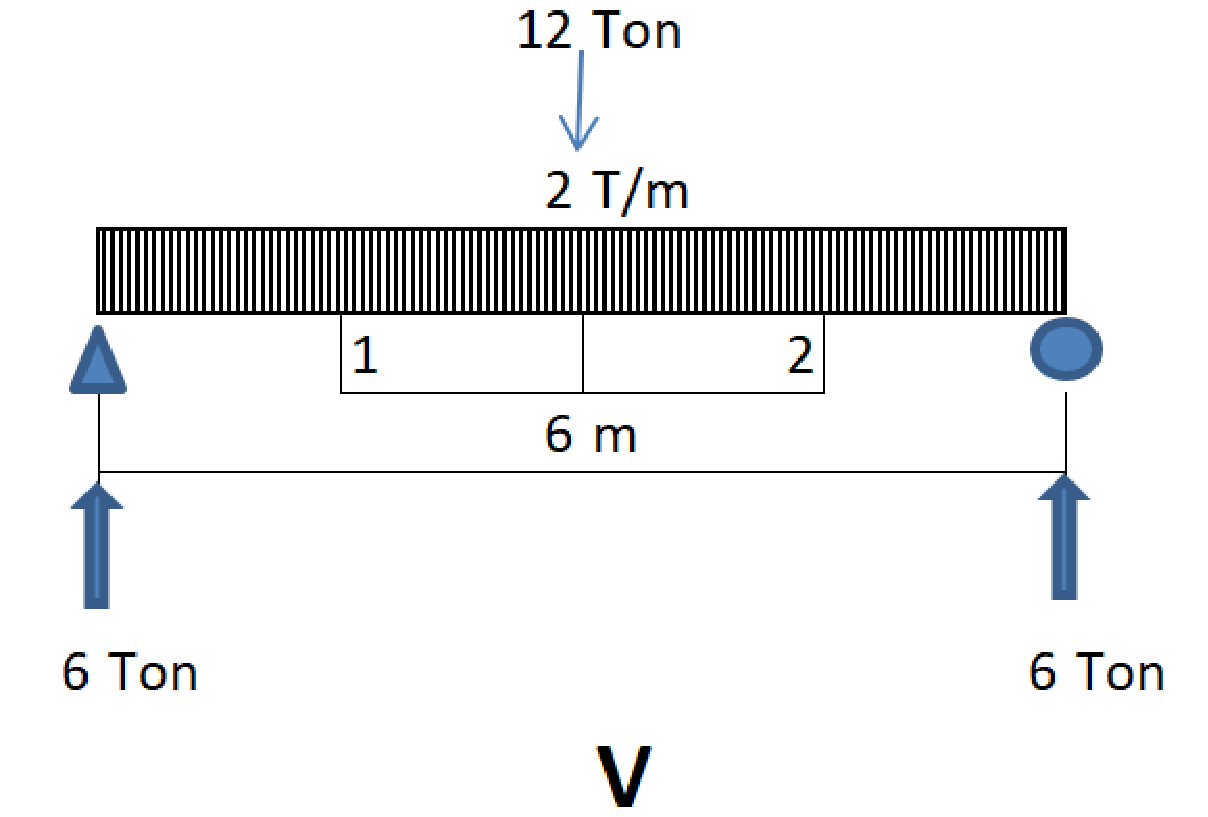
\includegraphics[width=0.5\textwidth]{mm22.pdf}
  \caption{Esquema del problema: Carga uniforme}
  \label{mm22}
\end{figure}
\textit{ Sol. }

Recordando que la fuerza se mide en toneladas, y el momentum en toneladas por metros.
\begin{figure}[h!]
\centering
  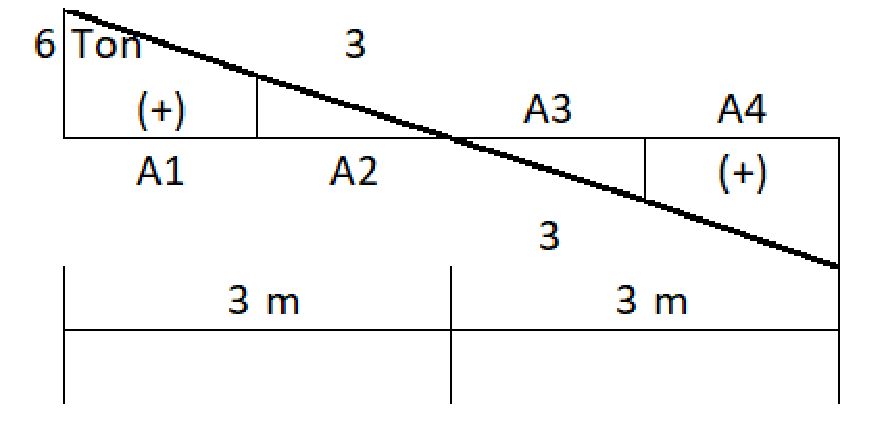
\includegraphics[width=0.5\textwidth]{mm23.pdf}
  \caption{Diagrama de cortantes}
  \label{mm23}
\end{figure}
De la figura \ref{mm23}, se puede ver que se genera dos triángulos opuestos por el vértice, pero al sumas sus áreas sería cero, pues son iguales pero de signos contrarios,
dividiéndolo en un cuatro partes, se tendrían dos trapecios y dos triángulos, de manera que se genera un diagrama de momentos (figura \ref{mm24|})
\begin{table}[h!]
    \centering
    \begin{tabular}{@{}ccccc@{}}
    \toprule
      & inte & M    & m     & int(Mm) \\ \midrule
      & 3    & 0    & 0     & 0       \\
    1 & 12   & 6.75 & 0.75  & 60.75   \\
      & 3    & 9    & 1.5   & 40.5    \\
      & 3    & 9    & 1.5   & 40.5    \\
    2 & 12   & 6.75 & 0.75  & 60.75   \\
      & 3    & 0    & 0     & 0       \\
      &      &      & suma: & 202.5   \\ \bottomrule
    \end{tabular}
    \caption{Áreas de los triángulos y trapecios}
    \label{tabmm8}
    \end{table}
\begin{figure}[h!]
\centering
  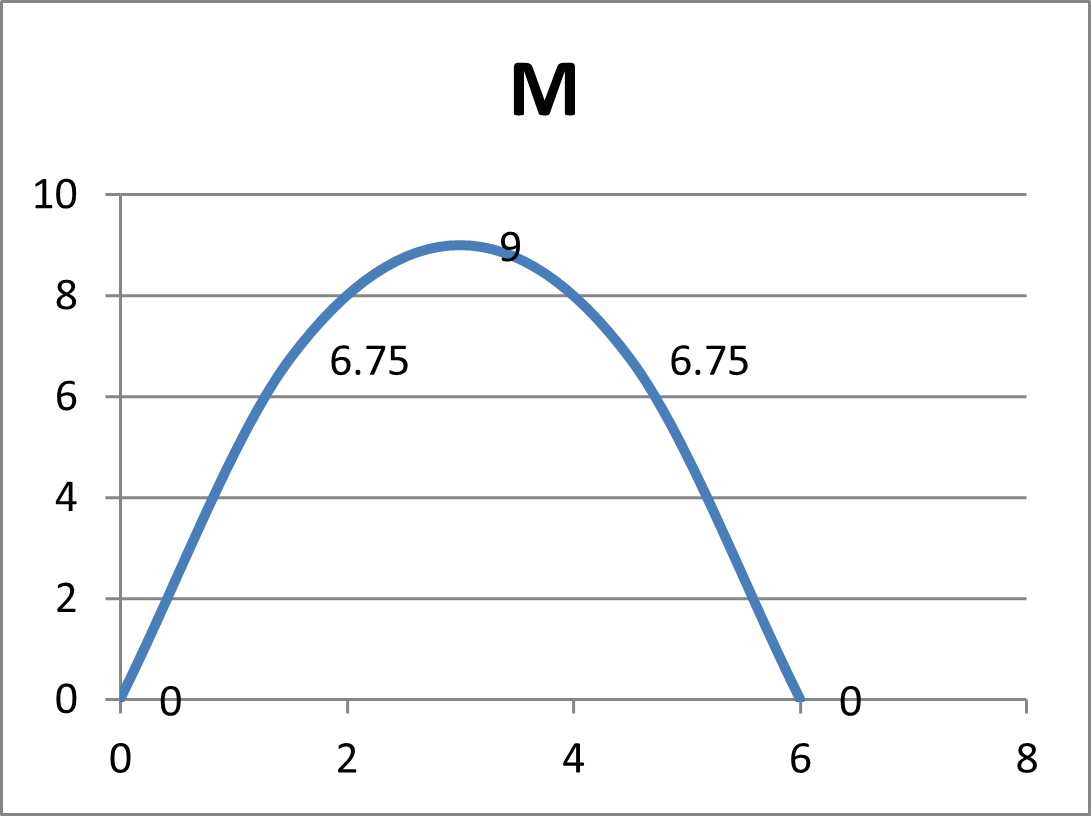
\includegraphics[width=0.5\textwidth]{mm24.png}
  \caption{Diagrama de momentos}
  \label{mm24}
\end{figure}
Observándose que es el comportamiento de éstas cuatro divisiones. Extrayendo el momento máximo $M=900000kg\cdot cm$, $y=cm$ obteniéndose $\sigma=1495.84kg/cm^2$, así la fuerza máxima es: $1518kg/cm^2$ los momentos de inercia están dados por un área de 0.1m de base y 0.19m por altura, así:
\begin{align*}
    I = 5.7\times 10^{5}m^4&& Es =2\times 10^7&&Es\cdot I = 1143.17&&Des = 0.02952m
\end{align*}
Para la obtención de éstos datos, es necesario ir al diagrama de fuerzas unitarias de la figura %\ref{mm25}:
% \begin{figure}[h!]
% \centering
%   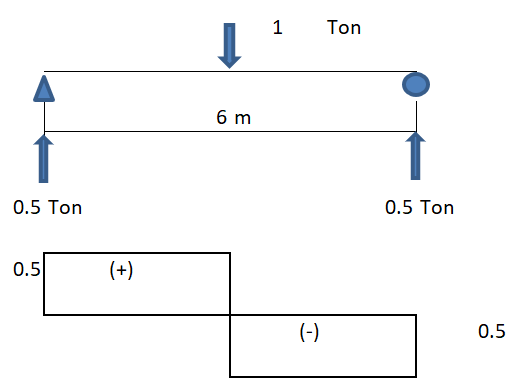
\includegraphics[width=0.5\textwidth]{mm25.pdf}
%   \caption{Diagrama de fuerzas unitarias}
%   \label{mm25}
% \end{figure}
El desplazamiento es relevante a la mitad de la viga, al ser una ecuación constante, es de primer grado, formándose la figura \ref{mm26}:
\begin{figure}[h!]
\centering
  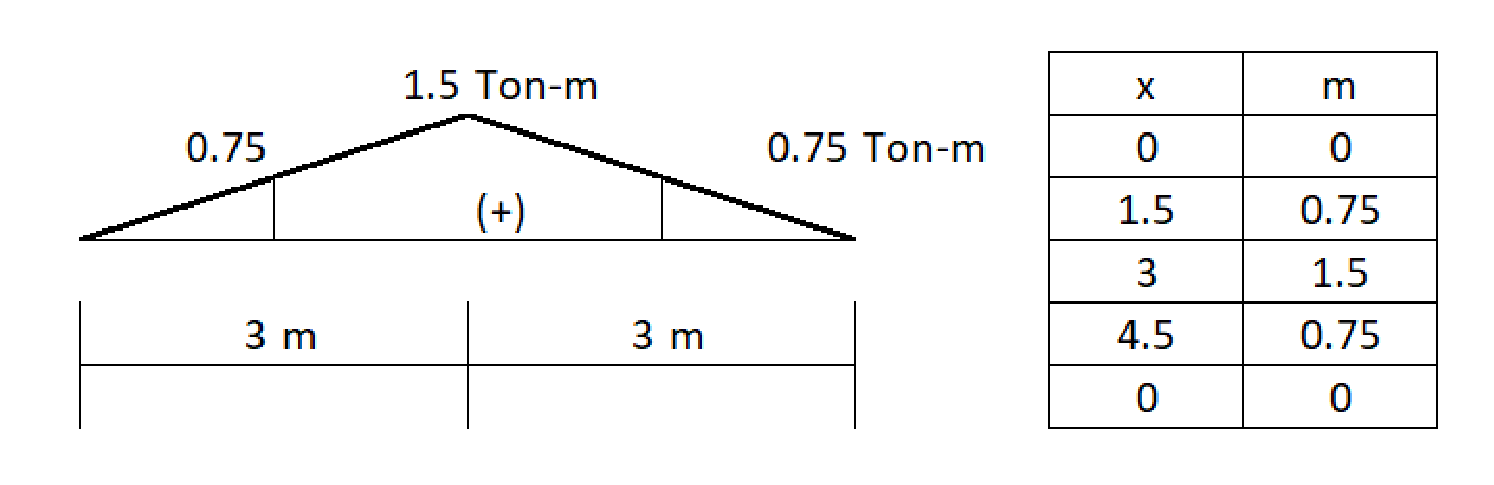
\includegraphics[width=0.5\textwidth]{mm26.pdf}
  \caption{Área de los trapecios}
  \label{mm26}
\end{figure}

Pero véase que aplicando la fórmula $Des=\frac{Suma}{6EI}$ de la tabla \ref{tabmm8}
\begin{align*}
    W = 2 \frac{T}{m}&& L = 6m&&E = 2\times 10^7&& I = 5.7\times 10^{ 5}m^4&&Des = 0.02952m
\end{align*}

% Resolver de nuevo a una viga hoja m. 

Del problema anterior, se calculará la ecuación tanto de fuerza cortante como de momento flexional.
De la figura
\begin{figure}[h!]
\centering
  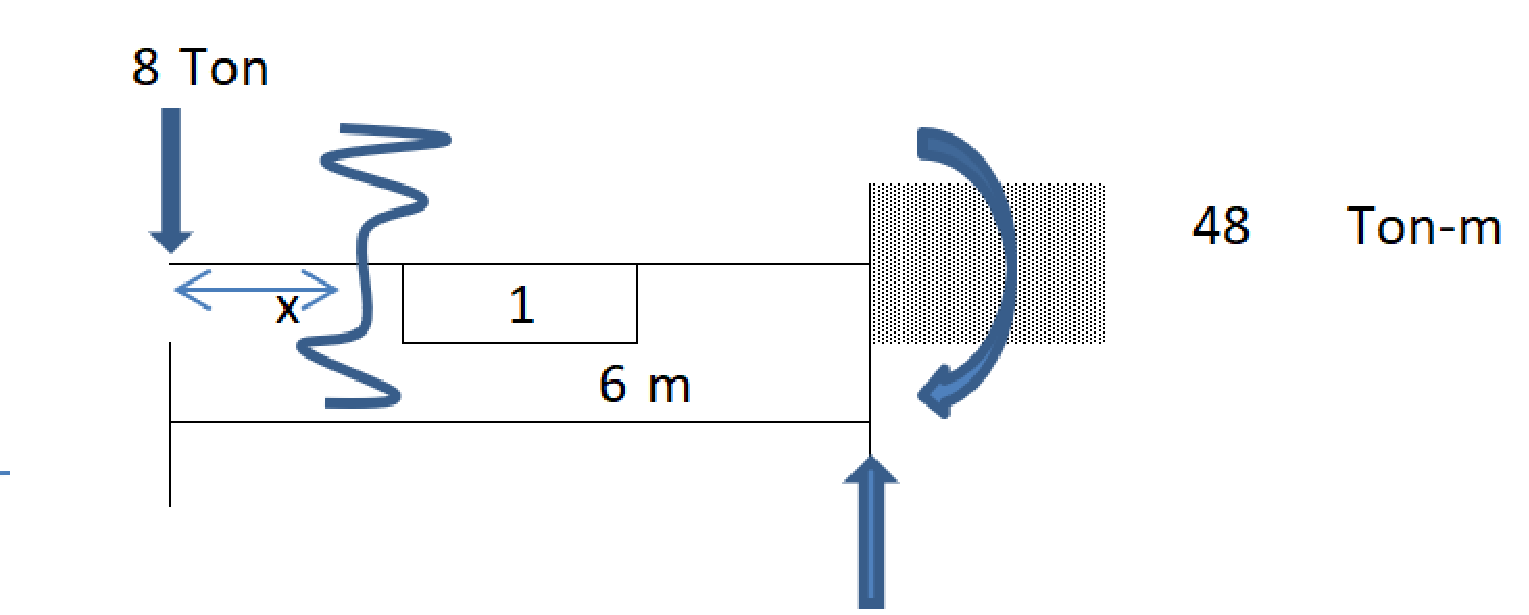
\includegraphics[width=0.5\textwidth]{mm27.pdf}
  \caption{Colocar una fuerza $x$ del extremo izquierdo}
  \label{mm27}
\end{figure}
De donde se puede notar que hay una fuerza actuante de 8 toneladas en la vertical, así la ecuación resultaría como $V-8$ Ton;
integrando aquella ecuación, se tiene que $V=-P$ así $M=-px$ y por lo tanto, $M=-8x$,
con esto se puede graficar fácilmente el diagrama de momento (Figura \ref{mm28})y el diagrama de cortantes (figura \ref{mm29}):
\begin{figure}[h!]
\centering
  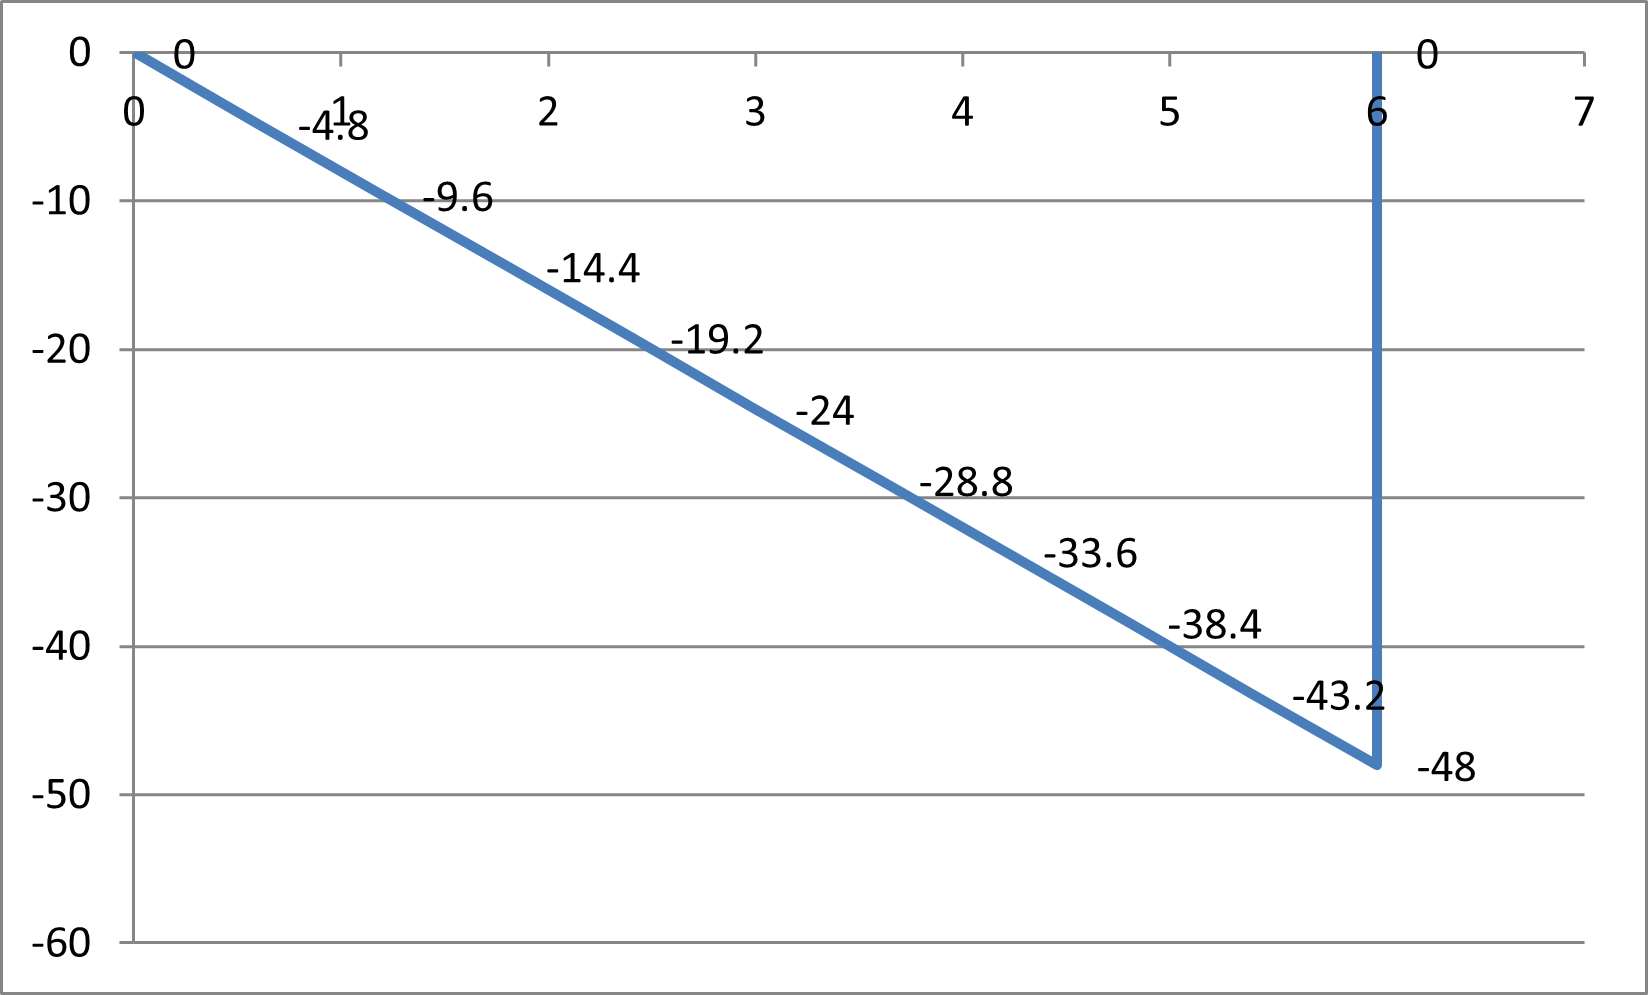
\includegraphics[width=0.5\textwidth]{mm28.png}
  \caption{Diagrama de momentos}
  \label{mm28}
\end{figure}
\begin{figure}[h!]
\centering
  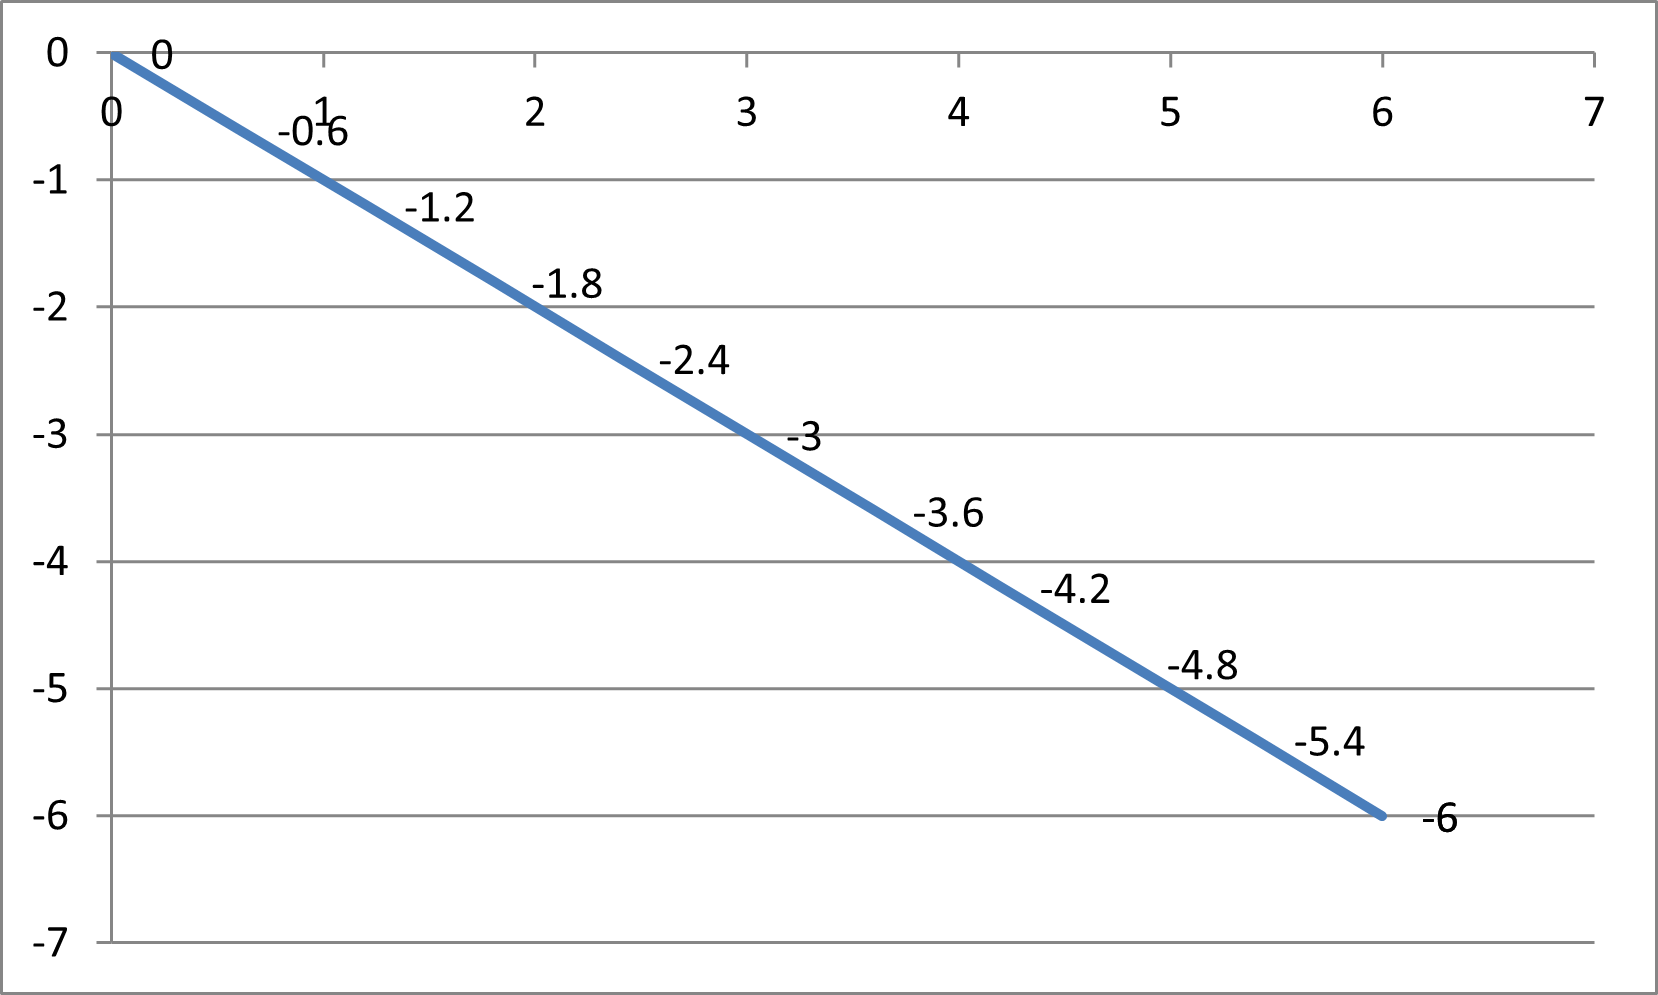
\includegraphics[width=0.5\textwidth]{mm29.png}
  \caption{Diagrama de cortantes}
  \label{mm29}
\end{figure}
Esto se puede hacer para cualquier viga, por ejemplo, en la figura \ref{mm30}, done hay una fuerza de 6 toneladas y en la carga uniforme es $2\cdot x$, de manera que la ecuación resulta $6-2x$.
\begin{figure}[h!]
\centering
  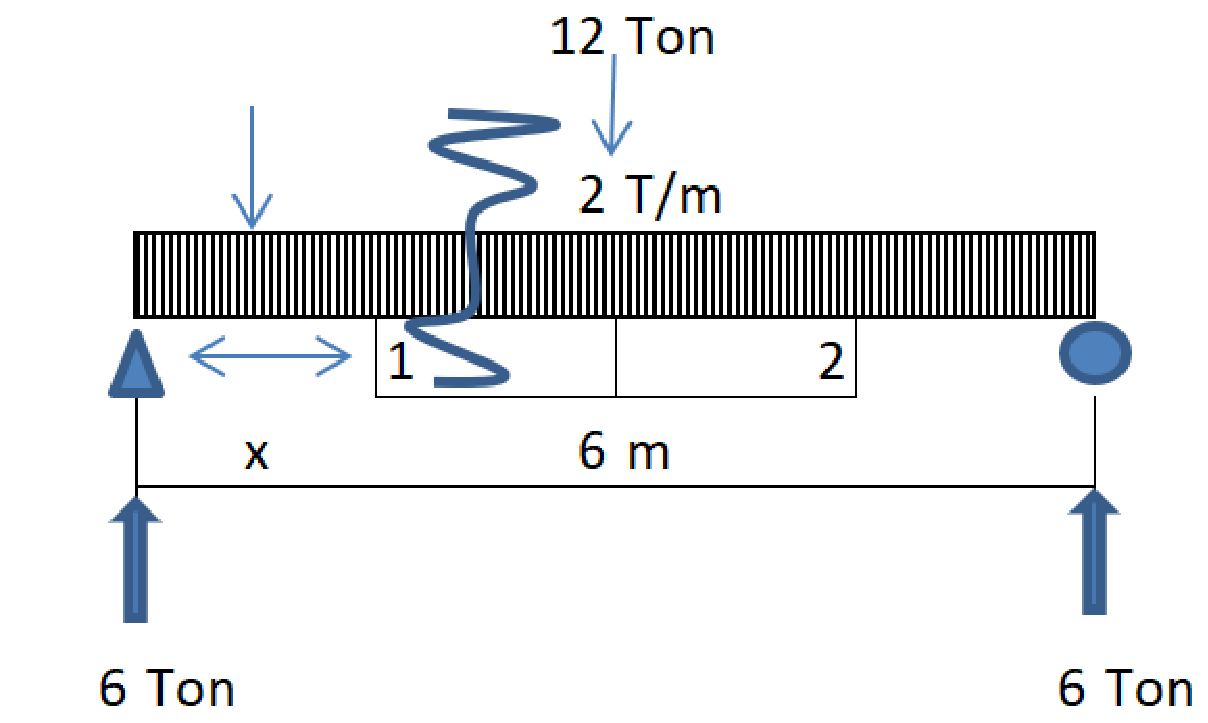
\includegraphics[width=0.5\textwidth]{mm30.pdf}
  \caption{Viga de ejemplo}
  \label{mm30}
\end{figure}
En éste caso particular, $V=6-2\cdot x$ al integrar, obtenemos $M=6x-\frac{2x^2}{2}$, graficándolas dividiendo a la viga en 10 partes, como se muestra en la figura \ref{mm31}:
\begin{figure}[h!]
\centering
  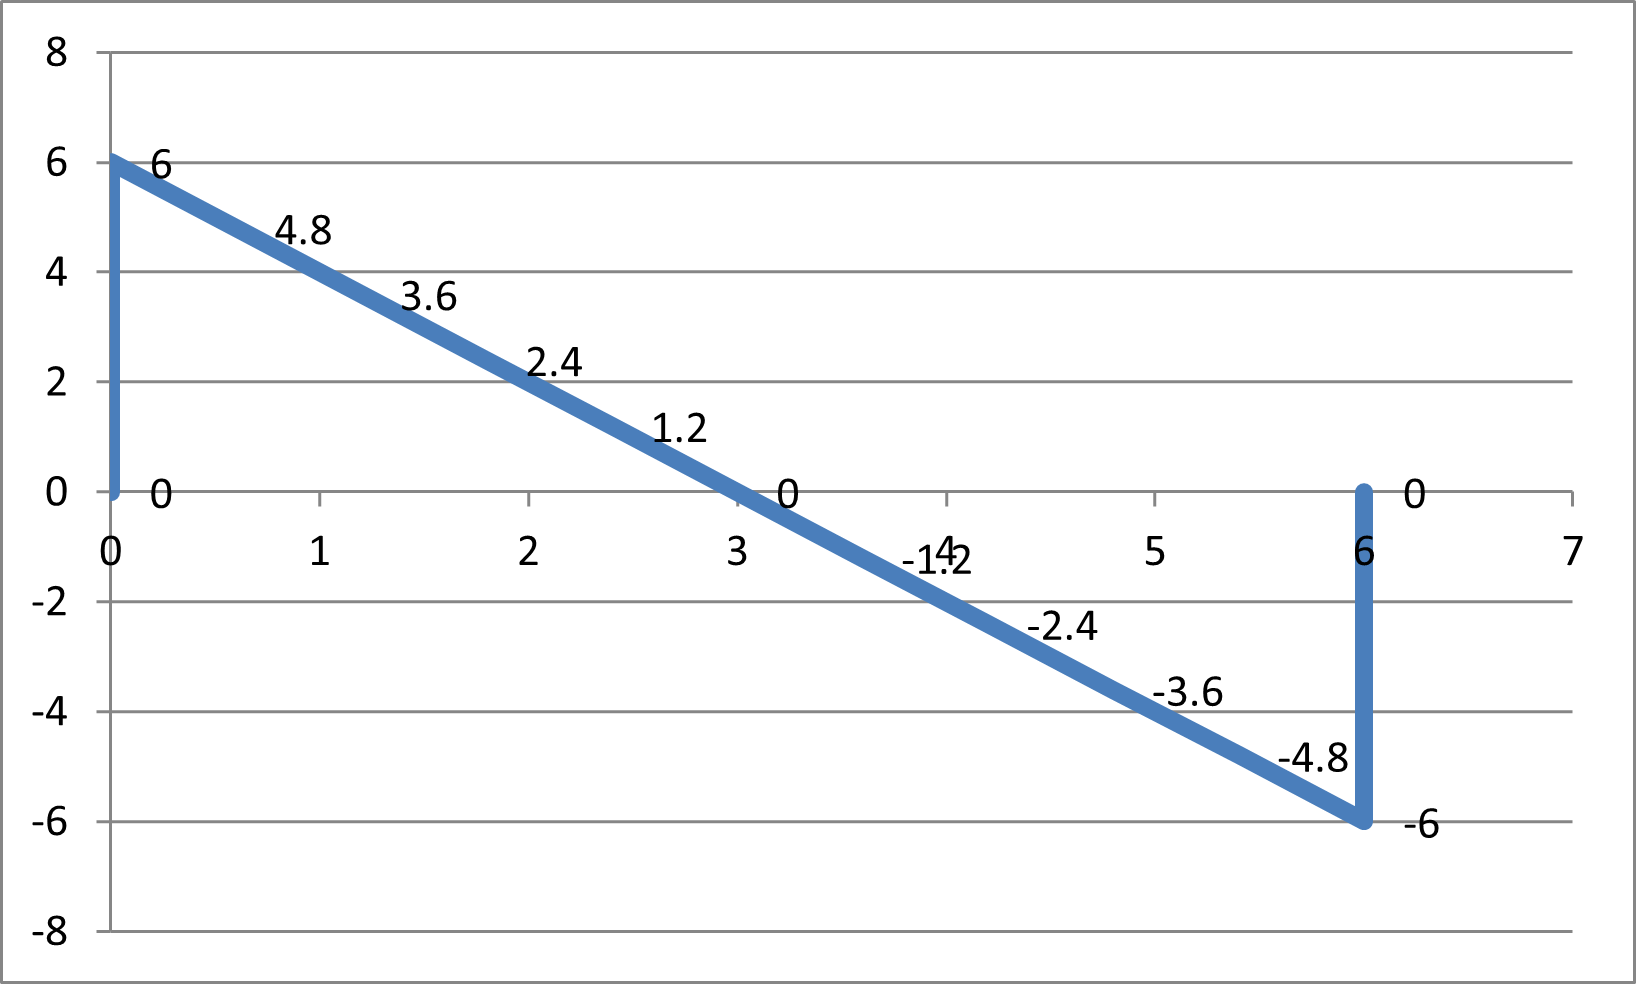
\includegraphics[width=0.5\textwidth]{mm31.png}
  \caption{Longitud de la viga con respecto 10 partes}
  \label{mm31}
\end{figure}
\begin{figure}[h!]
\centering
  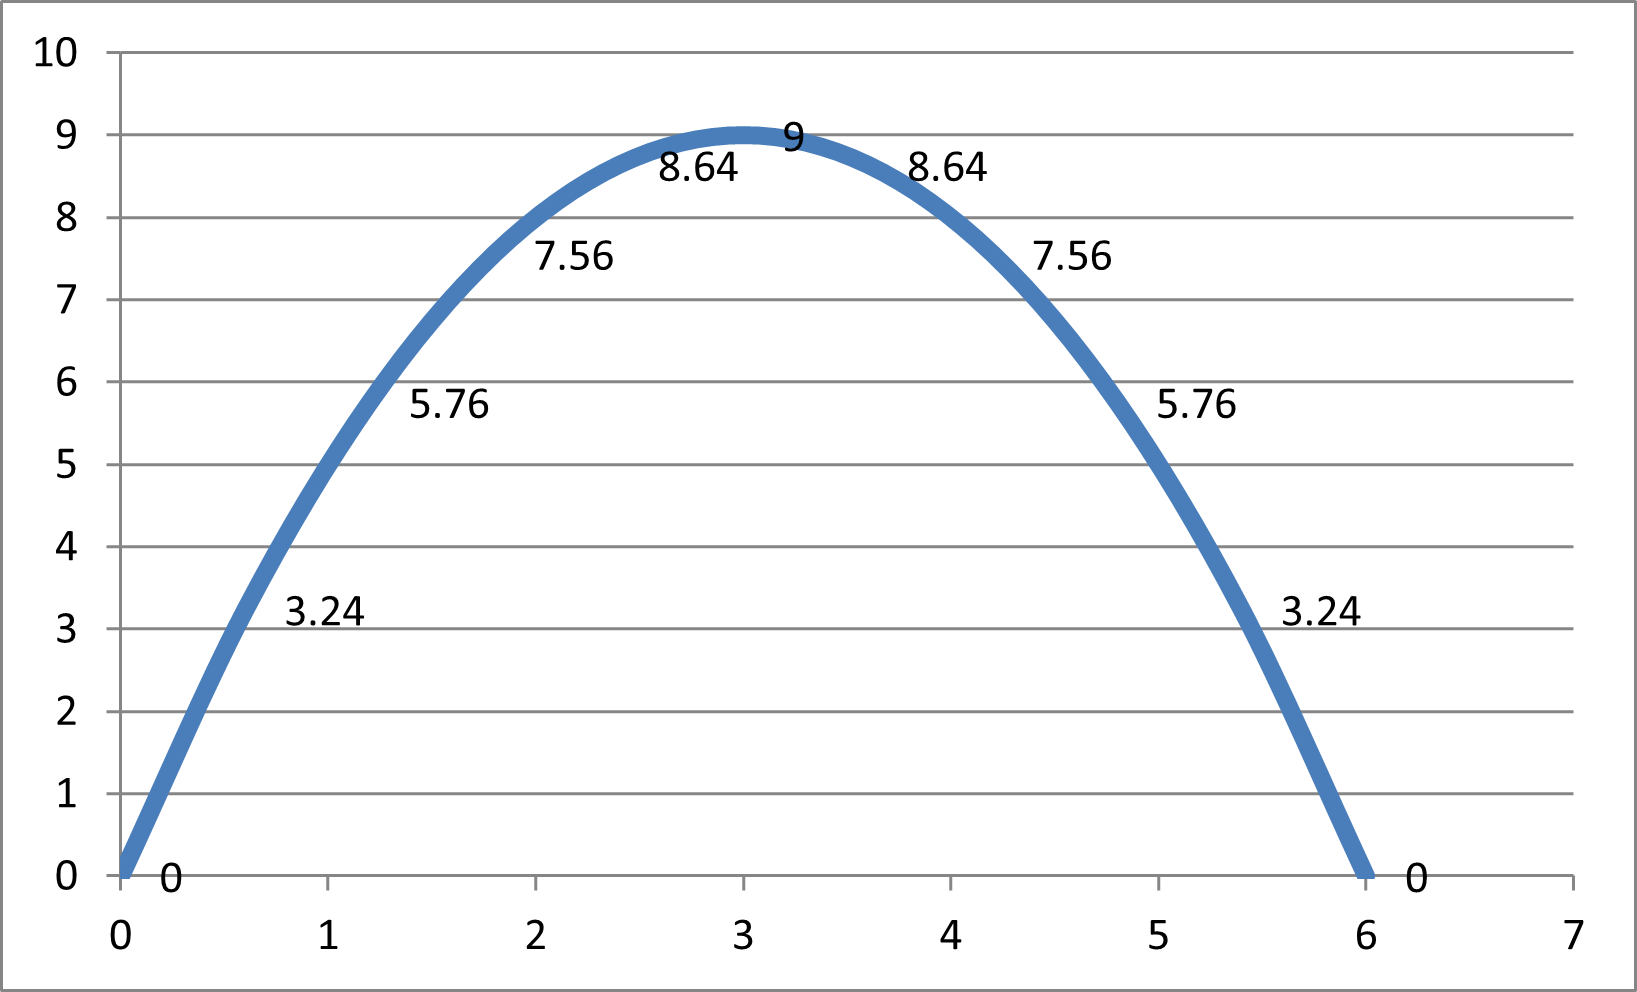
\includegraphics[width=0.5\textwidth]{mm32.png}
  \caption{Ecuación de momentos}
  \label{mm32}
\end{figure}
\begin{table}[h!]
    \centering
    \begin{tabular}{@{}cccc@{}}
    \toprule
    x   & V    & x                    & M                    \\ \midrule
    0   & 0    & 0                    & 0                    \\
    0   & 6    &                      &                      \\
    0.6 & 4.8  & 0.6                  & 3.24                 \\
    1.2 & 3.6  & 1.2                  & 5.76                 \\
    1.8 & 2.4  & 1.8                  & 7.56                 \\
    2.4 & 1.2  & 2.4                  & 8.64                 \\
    3   & 0    & 3                    & 9                    \\
    3.6 & -1.2 & 3.6                  & 8.64                 \\
    4.2 & -2.4 & 4.2                  & 7.56                 \\
    4.8 & -3.6 & 4.8                  & 5.76                 \\
    5.4 & -4.8 & 5.4                  & 3.24                 \\
    6   & -6   & \multicolumn{1}{l}{} & \multicolumn{1}{l}{} \\
    6   & 0    & 6                    & 0                    \\ \bottomrule
    \end{tabular}
    \caption{Ecuación de momentos y la recta en la viga}
    \label{tabmm888}
\end{table}
Con esto en contexto, se procede a realizar el siguiente problema propuesto:
\begin{problem}
    \begin{figure}[h!]
    \centering
      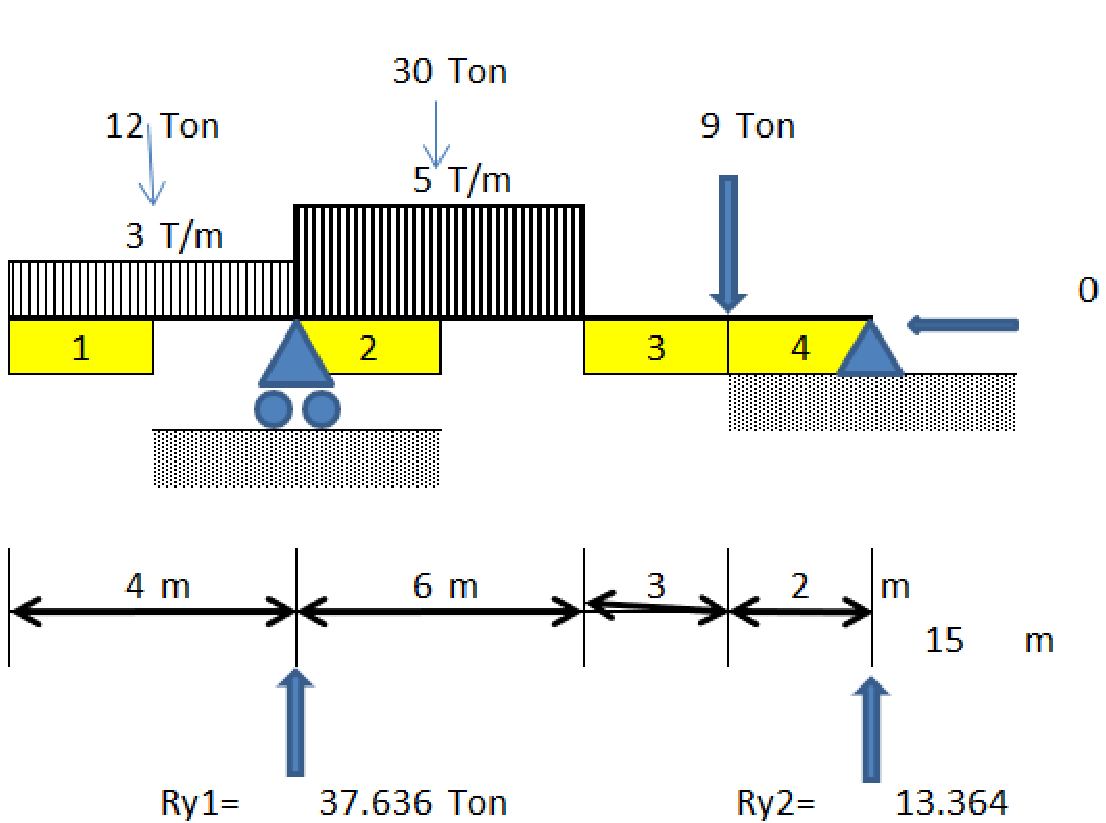
\includegraphics[width=0.5\textwidth]{mm33.pdf}
      \caption{Esquema del problema}
      \label{mm33}
    \end{figure}
\end{problem}

\textit{ Sol. }

Del esquema anterior, $V=-wx$ integrando quedaría como $M=-wx^2/2$ $M=-3\cdot x^2/2$, dibujando el diagrama de cortantes quedaría como en la figura \ref{mm34}
\begin{figure}[h!]
\centering
  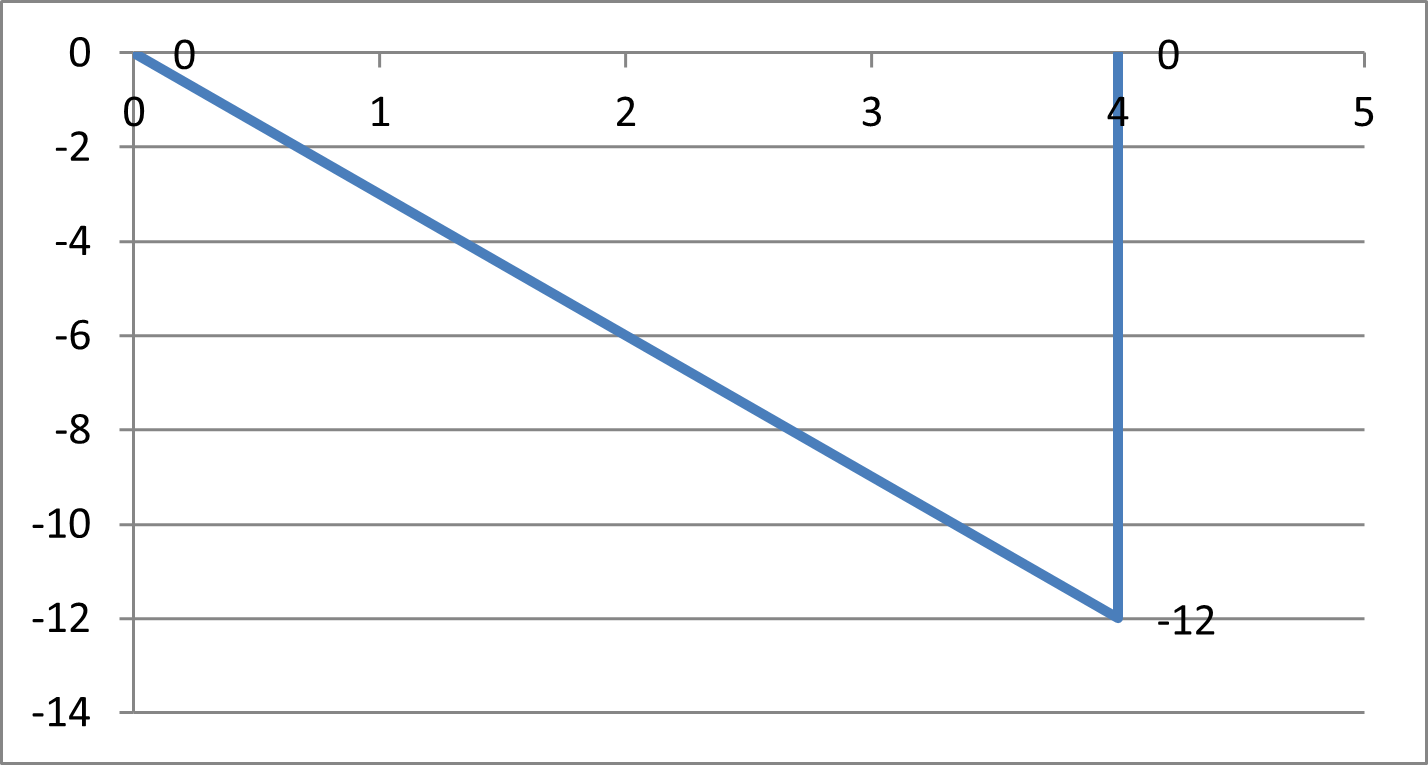
\includegraphics[width=0.5\textwidth]{mm34.png}
  \caption{Diagrama de Cortantes}
  \label{mm34}
\end{figure}
En la figura anterior ya tiene la suma de momentos, en los nudos junto con la suma de fuerzas;
si se comparan las fuerzas de 12 toneladas en la vertical superior contra los 37.636 Ton restándoles nos da el 25.636 de la figura \ref{mm35}
\begin{figure}[h!]
\centering
  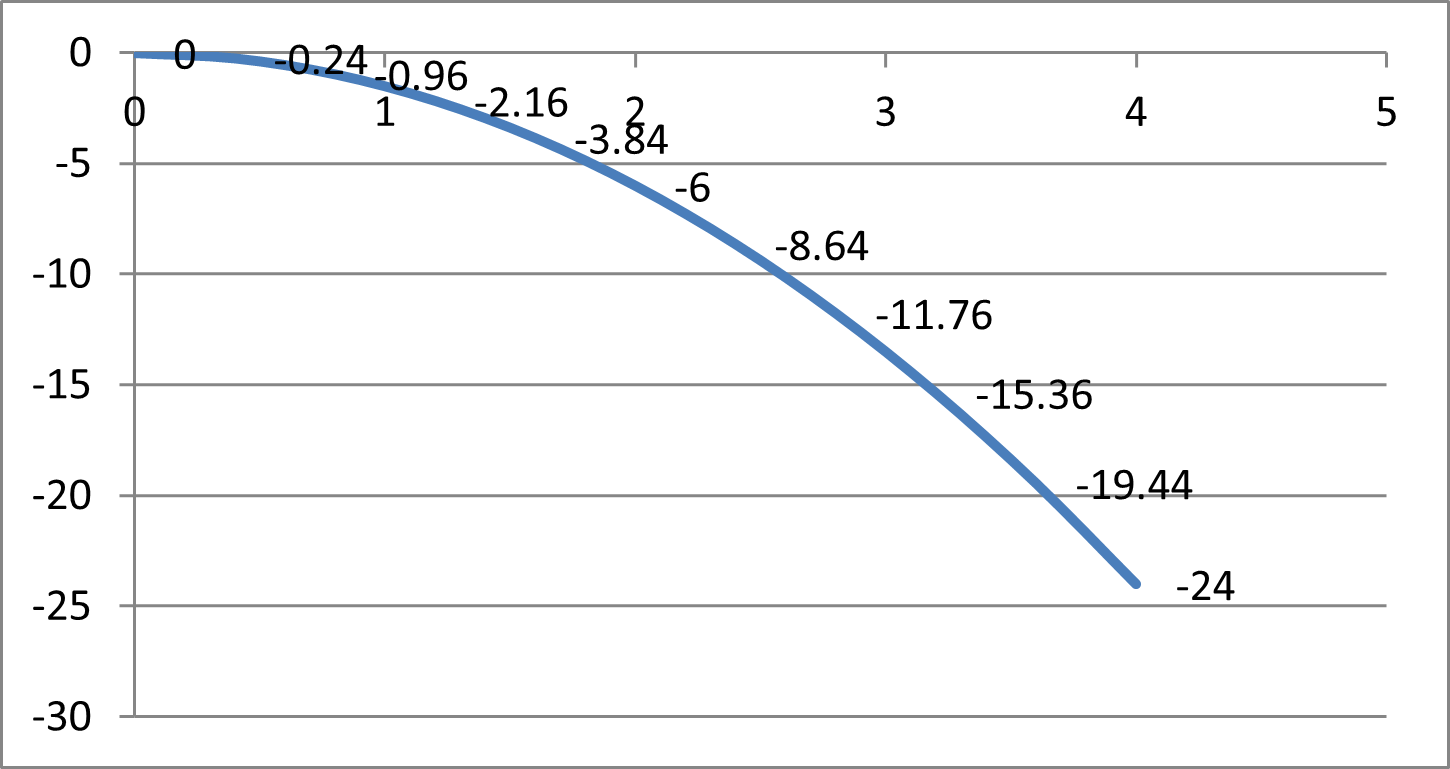
\includegraphics[width=0.5\textwidth]{mm35.png}
  \caption{Suma de fuerzas}
  \label{mm35}
\end{figure}
El último momento de la barra anterior es el 24, para calcular el diagrama de constantes y momentos, véase la barra de una manera ampliada en la figura \ref{mm37}
\begin{figure}[h!]
\centering
  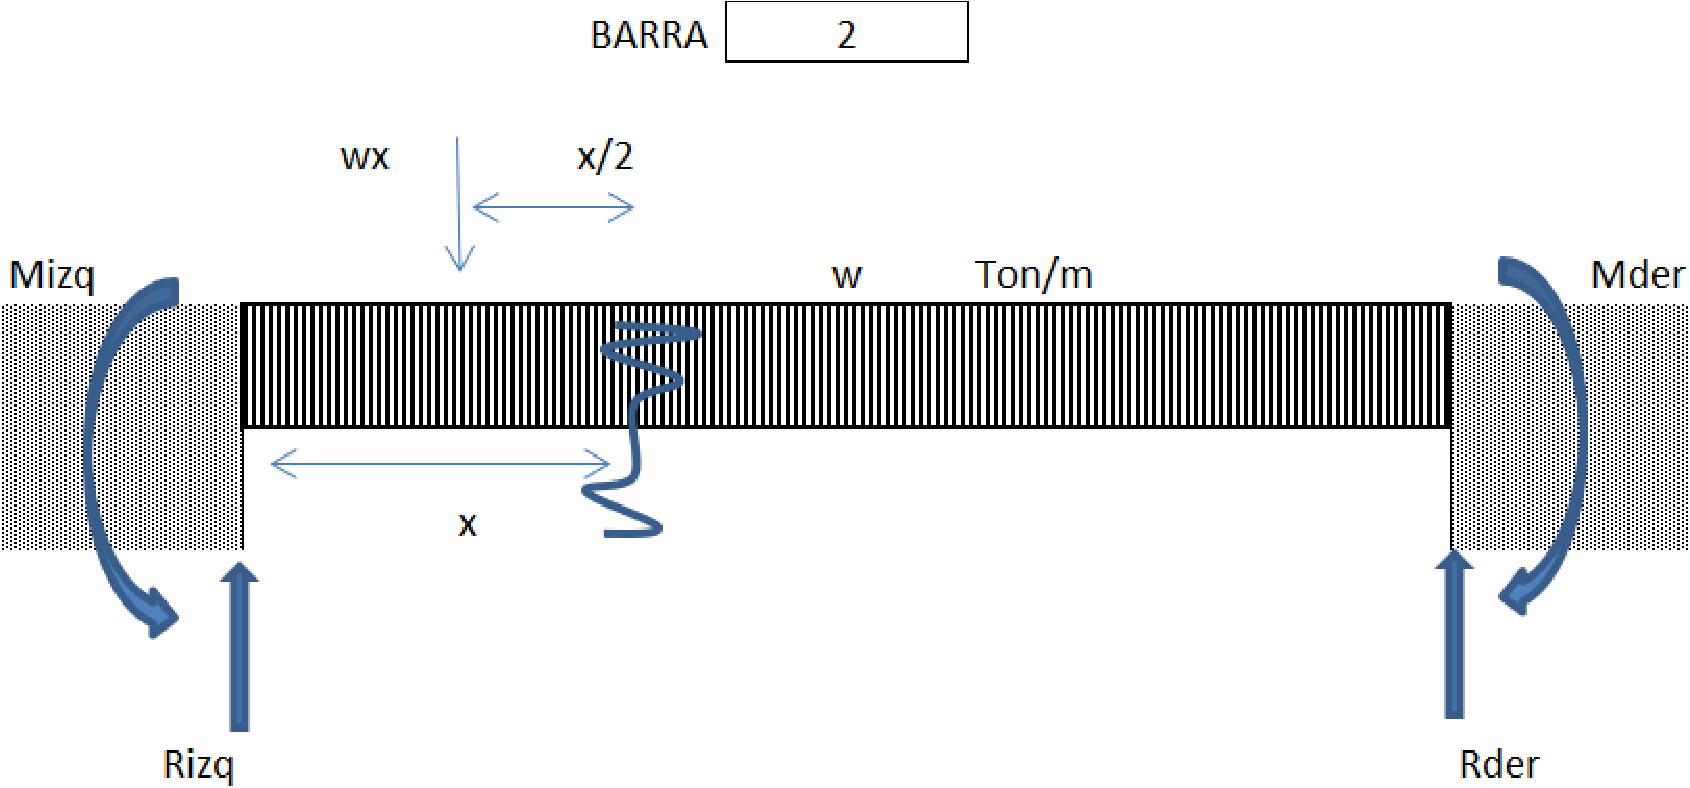
\includegraphics[width=0.5\textwidth]{mm37.pdf}
  \caption{Barra amplificada}
  \label{mm37}
\end{figure}
La reacción es positiva y negativa es la carga $ws$ Véase que las ecuaciones que se generan son:
\begin{align*}
    &V = R_{izq} - wx\\
    &M = R_{izq}(x) -w\left(\frac{x^2}{2}\right) - M_{izq}
\end{align*}
Aplicando las ecuaciones anteriores, modelamos en la figura \ref{mm38}
\begin{figure}[h!]
\centering
  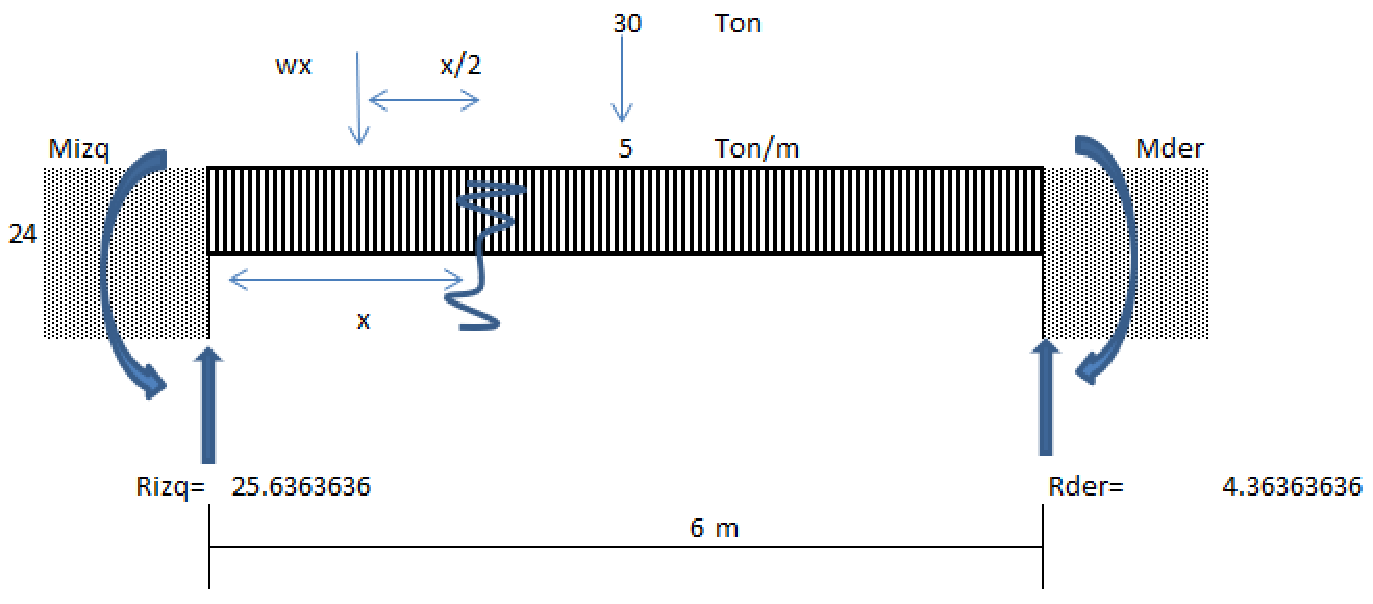
\includegraphics[width=0.5\textwidth]{mm38.pdf}
  \caption{Barra dos}
  \label{mm38}
\end{figure}
Obtenemos las siguientes gráficas de la tabla \ref{tabmm9}
\begin{table}[h!]
    \centering
    \begin{tabular}{@{}cccc@{}}
    \toprule
    x   & V      & x   & M       \\ \midrule
    0   & 0      & 0   & -24.000 \\
    0   & 25.636 & 0.6 & -9.518  \\
    0.6 & 22.636 & 1.2 & 3.164   \\
    1.2 & 19.636 & 1.8 & 14.045  \\
    1.8 & 16.636 & 2.4 & 23.127  \\
    2.4 & 13.636 & 3   & 30.409  \\
    3   & 10.636 & 3.6 & 35.891  \\
    3.6 & 7.636  & 4.2 & 39.573  \\
    4.2 & 4.636  & 4.8 & 41.455  \\
    4.8 & 1.636  & 5.4 & 41.536  \\
    5.4 & -1.364 & 6   & 39.818  \\
    6   & -4.364 &     &         \\
    6   & 0      &     &         \\ \bottomrule
    \end{tabular}
    \caption{Gráficas de cortantes }
    \label{tabmm9}
\end{table}
\begin{figure}[h!]
\centering
  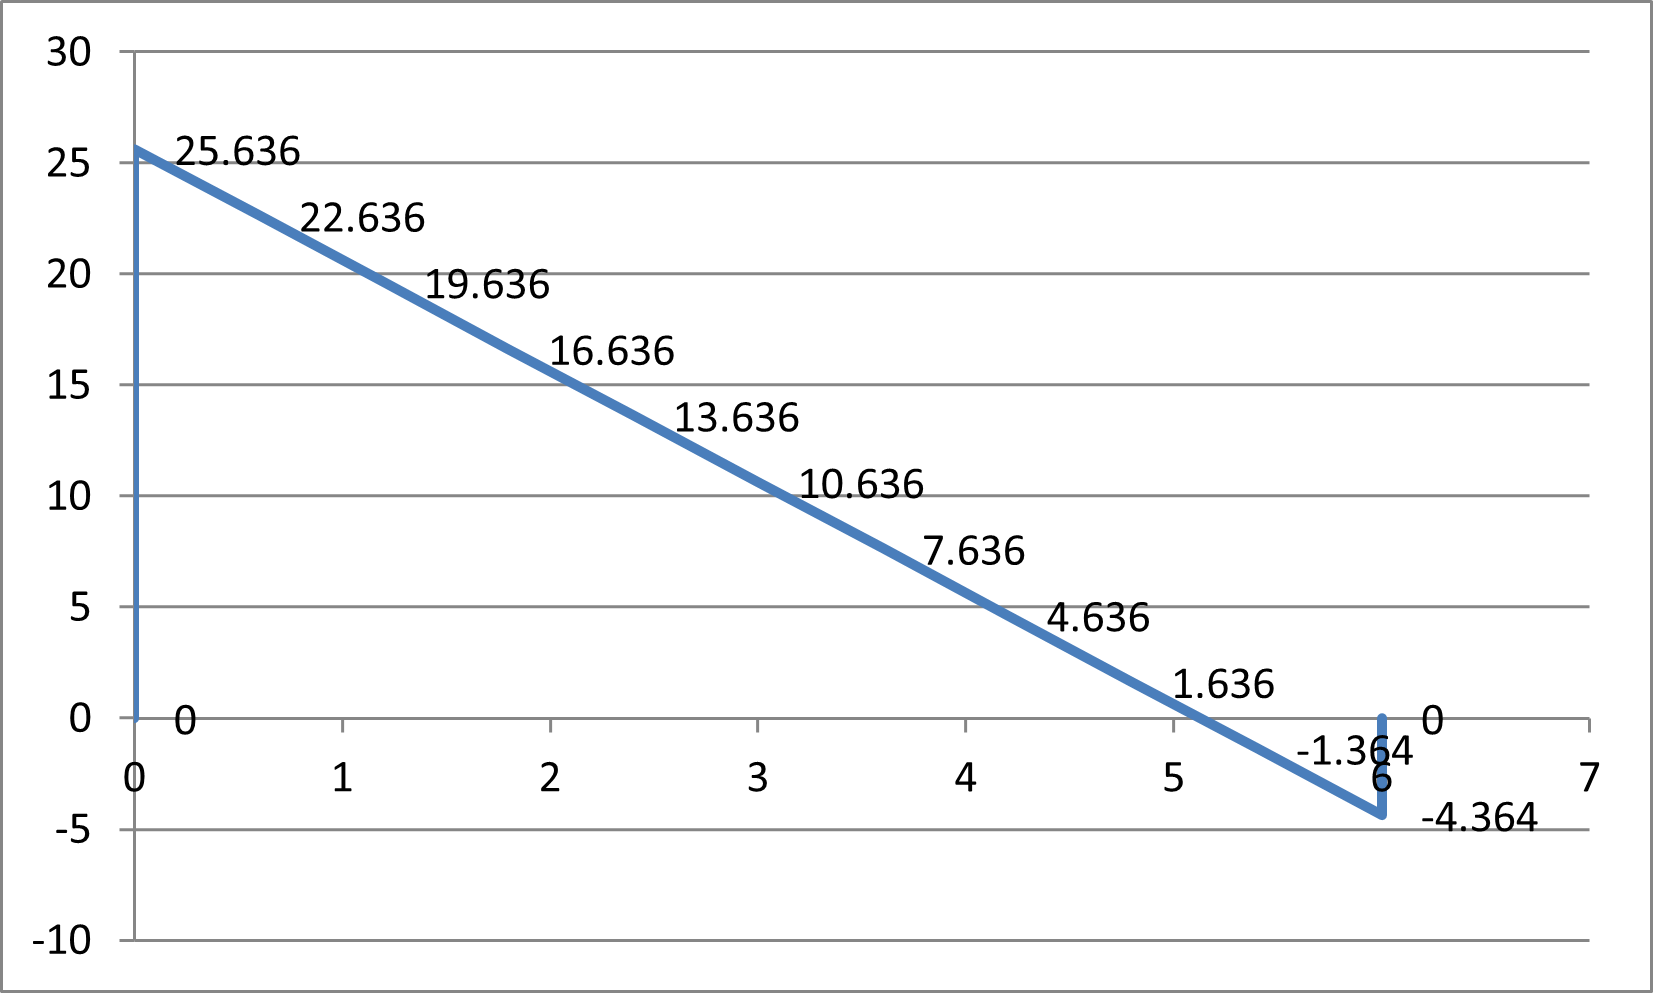
\includegraphics[width=0.5\textwidth]{mm39.png}
  \caption{Diagrama de cortantes}
  \label{mm39}
\end{figure}
De aquí sabiendo que $V=0$, x=5.1272 y el momento máximo $M_{max}=41.7223$
\begin{figure}[h!]
\centering
  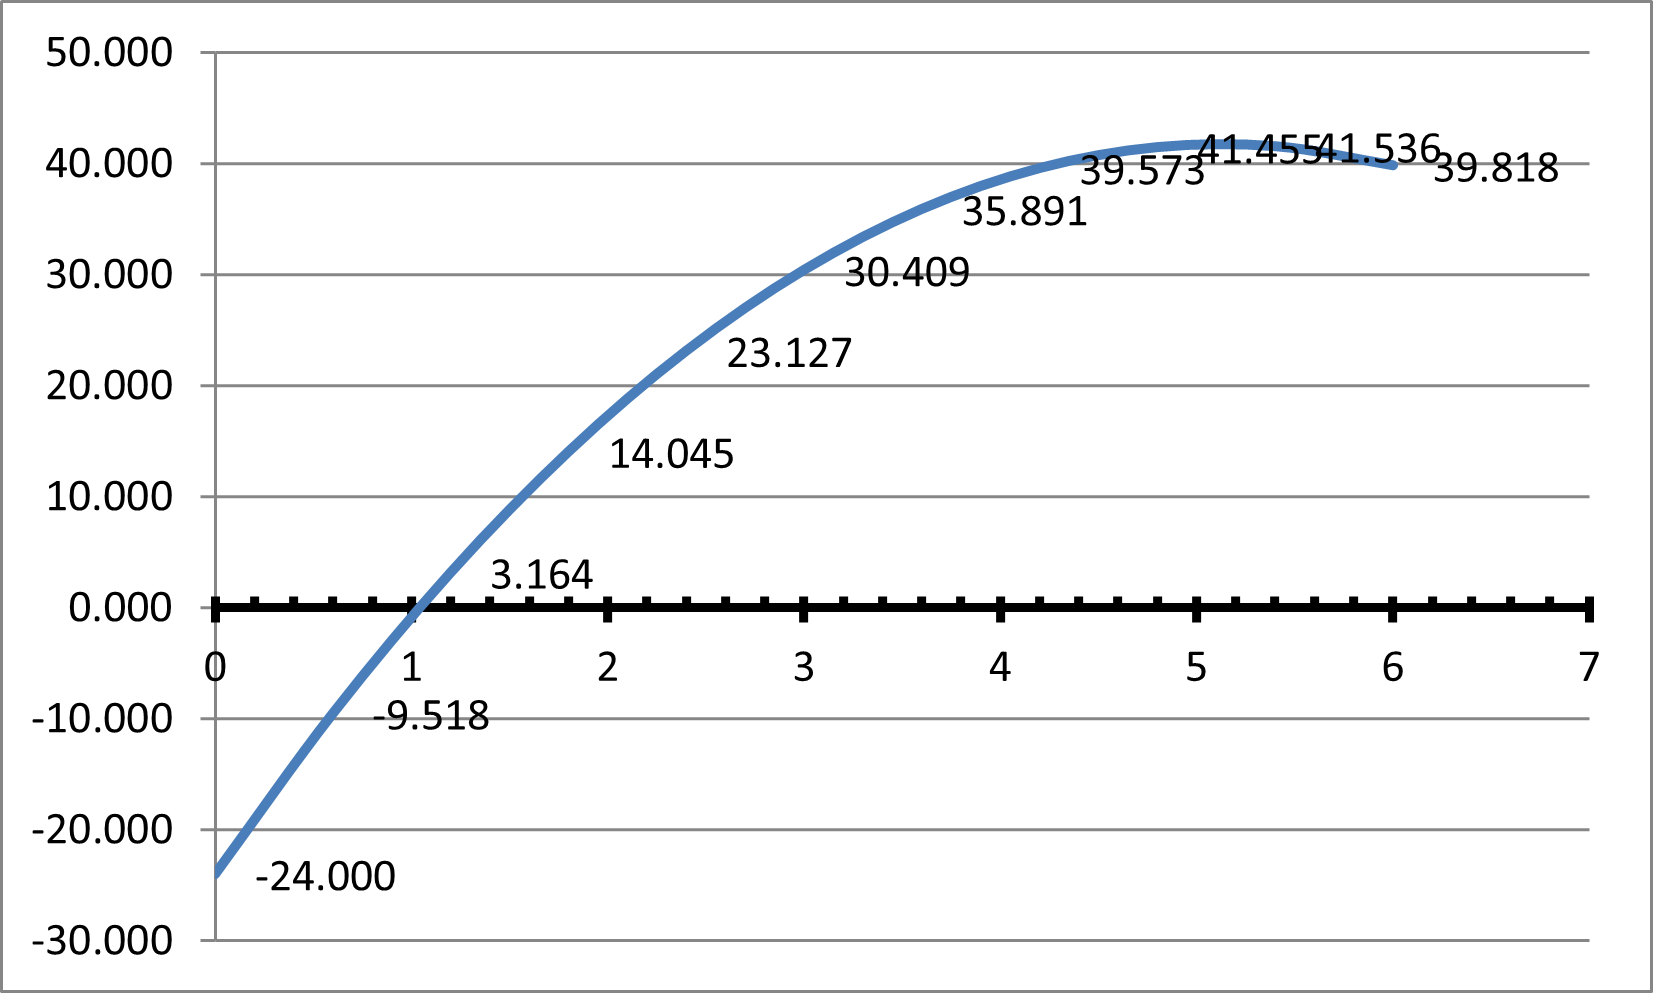
\includegraphics[width=0.5\textwidth]{mm40.png}
  \caption{Diagrama}
  \label{mm40}
\end{figure}
Aplicando el mismo procedimiento para el tramo tres y cuatro obtenemos:
\begin{figure}[h!]
\centering
  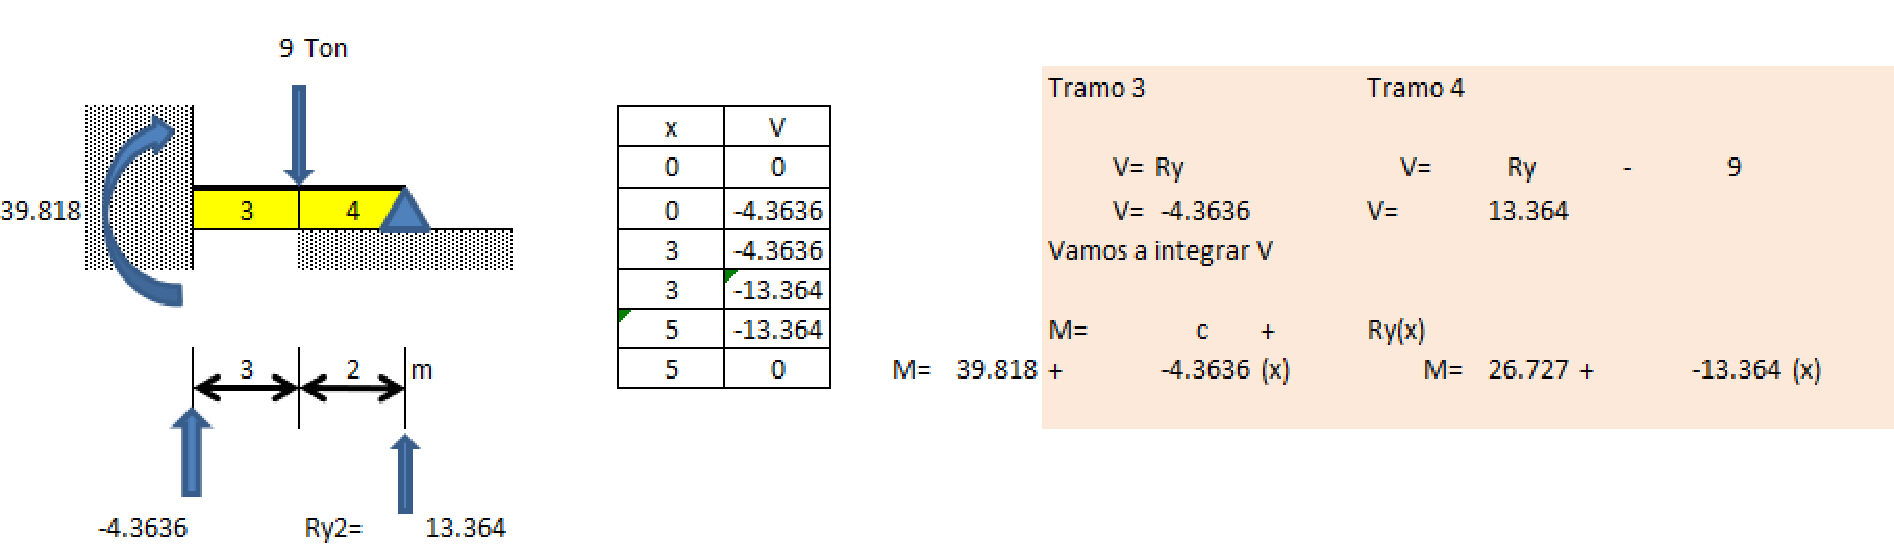
\includegraphics[width=0.5\textwidth]{mm41.pdf}
  \caption{Tabulación de fuerzas cortantes}
  \label{mm41}
\end{figure}
Esto genera rectas porque no tiene cargas interiores
\begin{figure}[h!]
\centering
  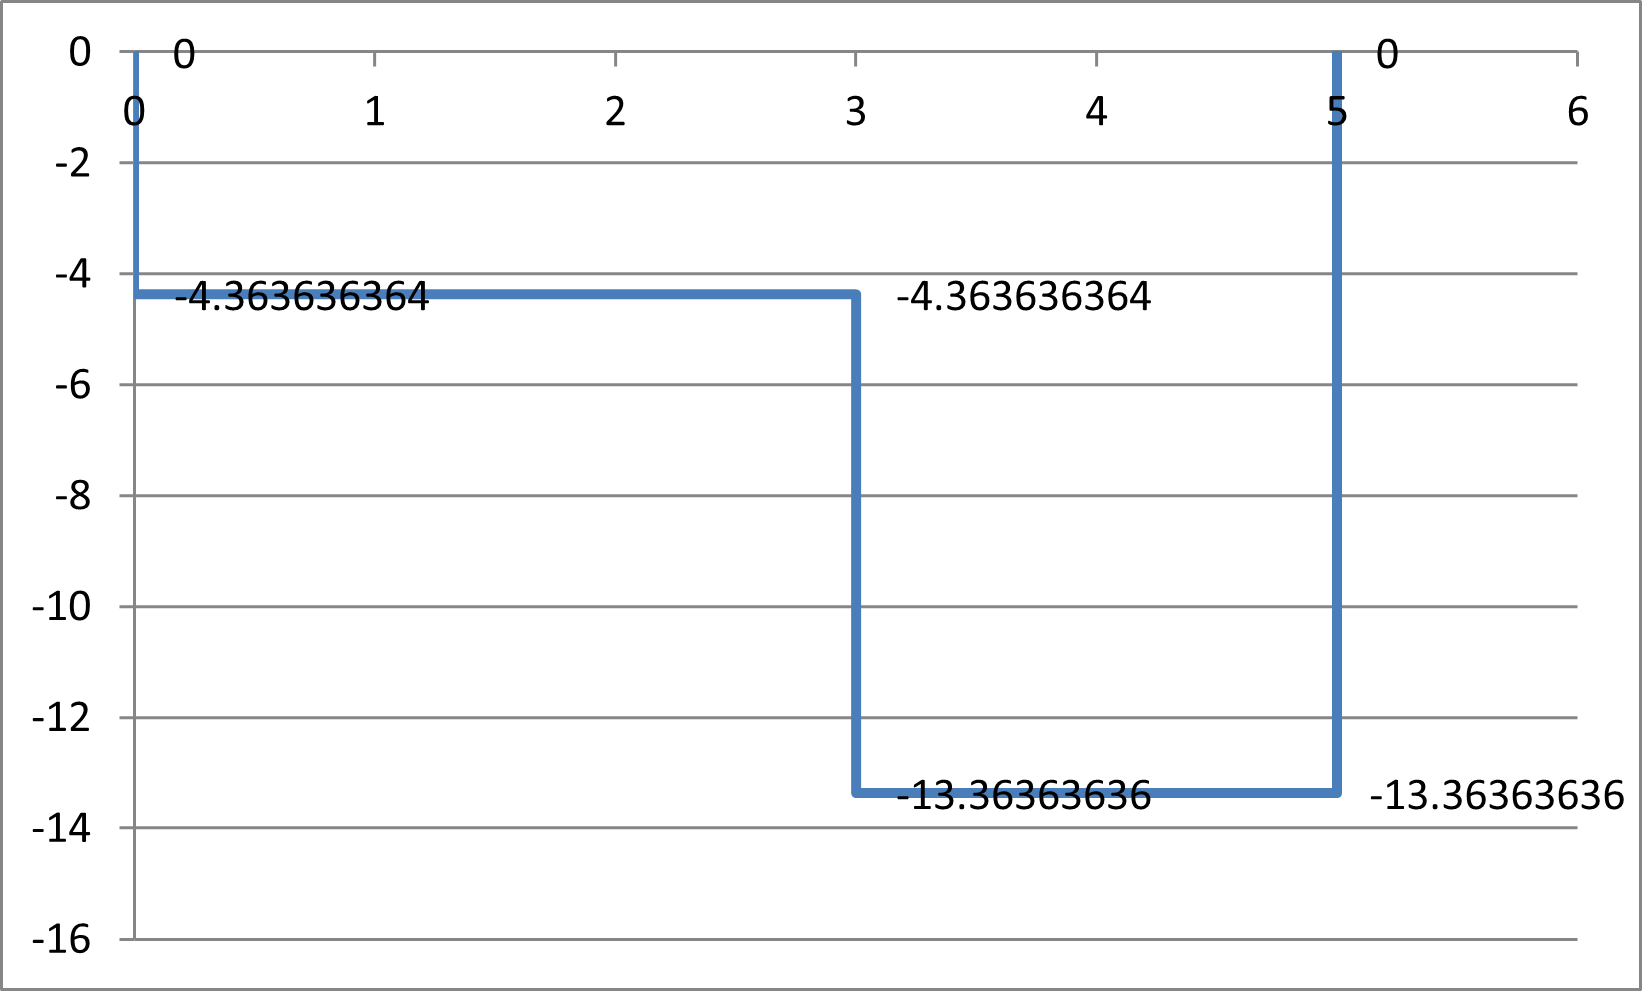
\includegraphics[width=0.5\textwidth]{mm42.png}
  \caption{Máxima fuerza cortante}
  \label{mm42}
\end{figure}
Así que recopilando todos los cálculos obtenemos el diagrama de cortantes 
\begin{figure}[h!]
\centering
  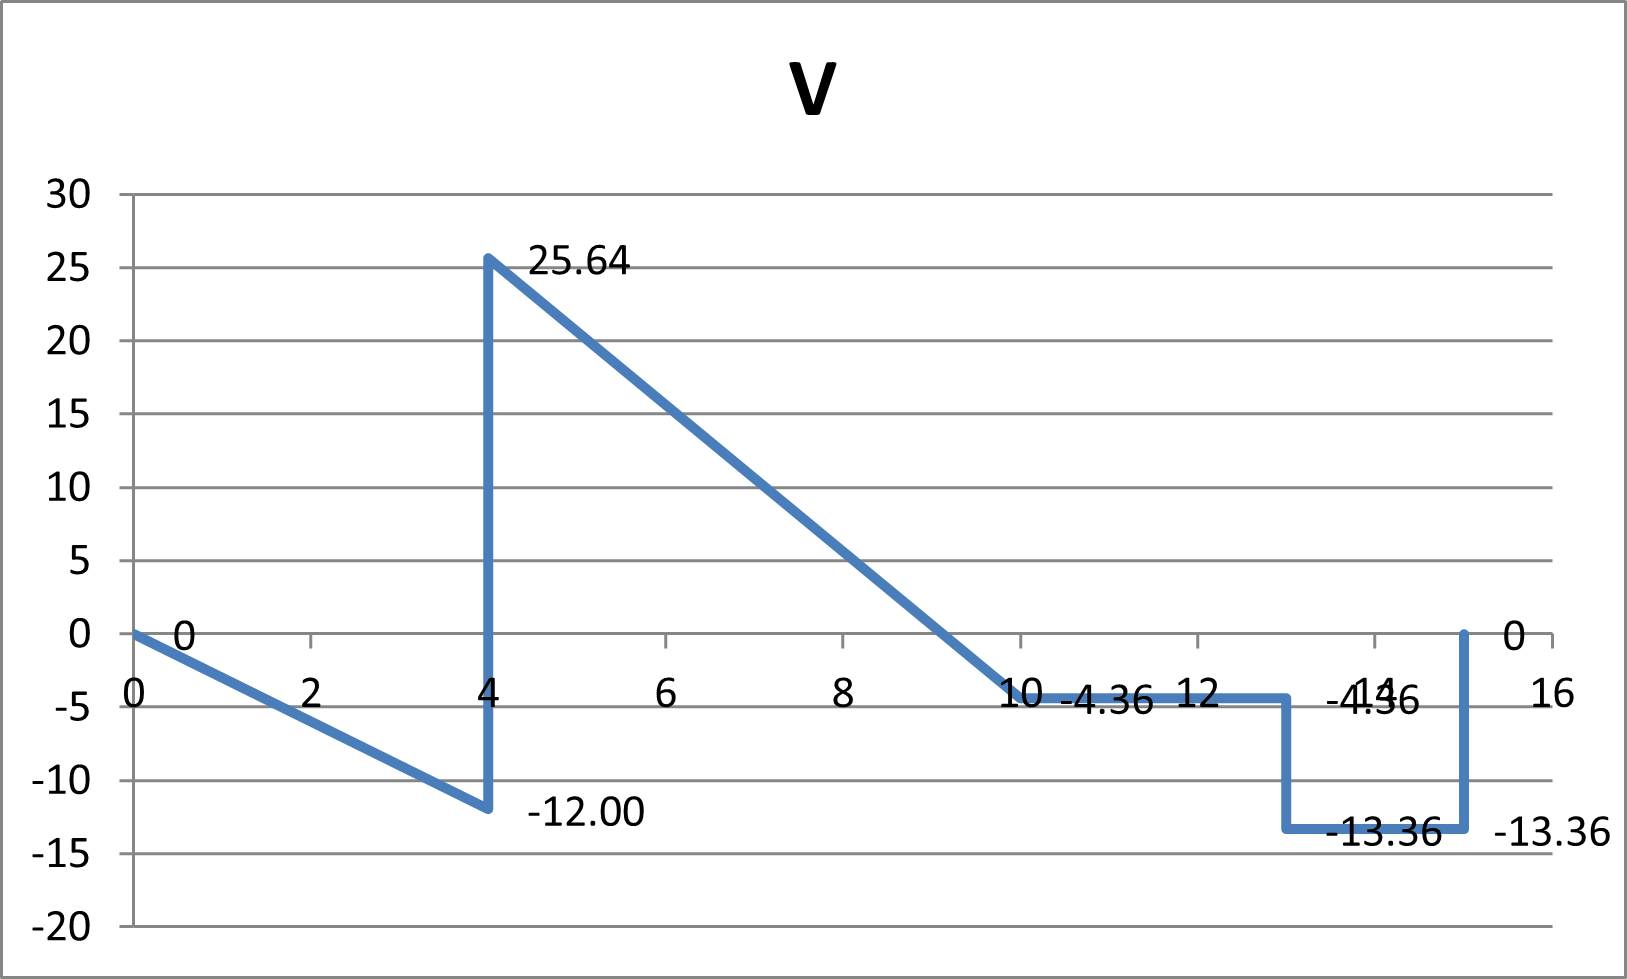
\includegraphics[width=0.5\textwidth]{mm43.png}
  \caption{Diagrama de cortantes}
  \label{mm43}
\end{figure}
\begin{figure}[h!]
\centering
  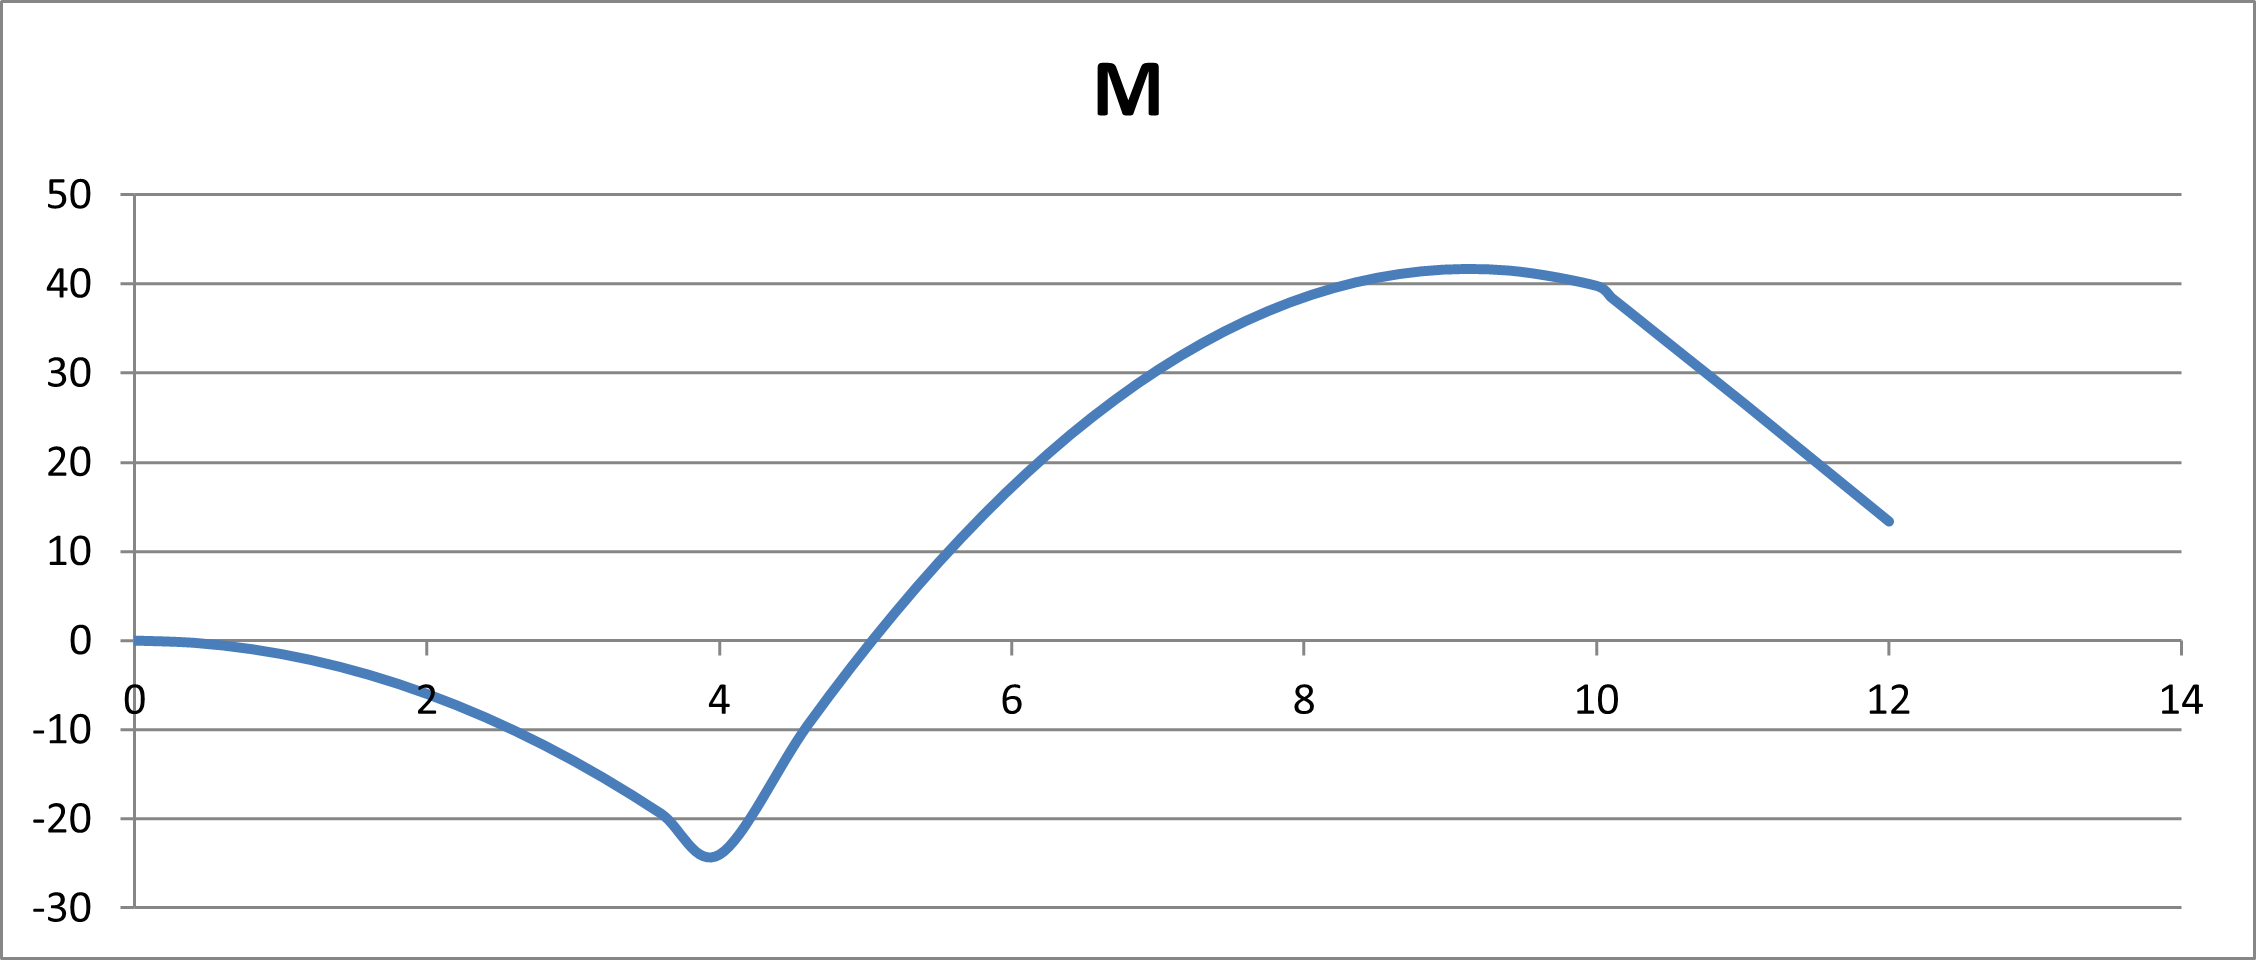
\includegraphics[width=0.5\textwidth]{mm44.png}
  \caption{Diagrama de momentos}
  \label{mm44}
\end{figure}
Al ser demasiados datos, no se colocaron números para poder apreciar la curva y rectas, más fácil de comprender en la imágen obtenida del programa de SAP2000:
\begin{figure}[h!]
\centering
  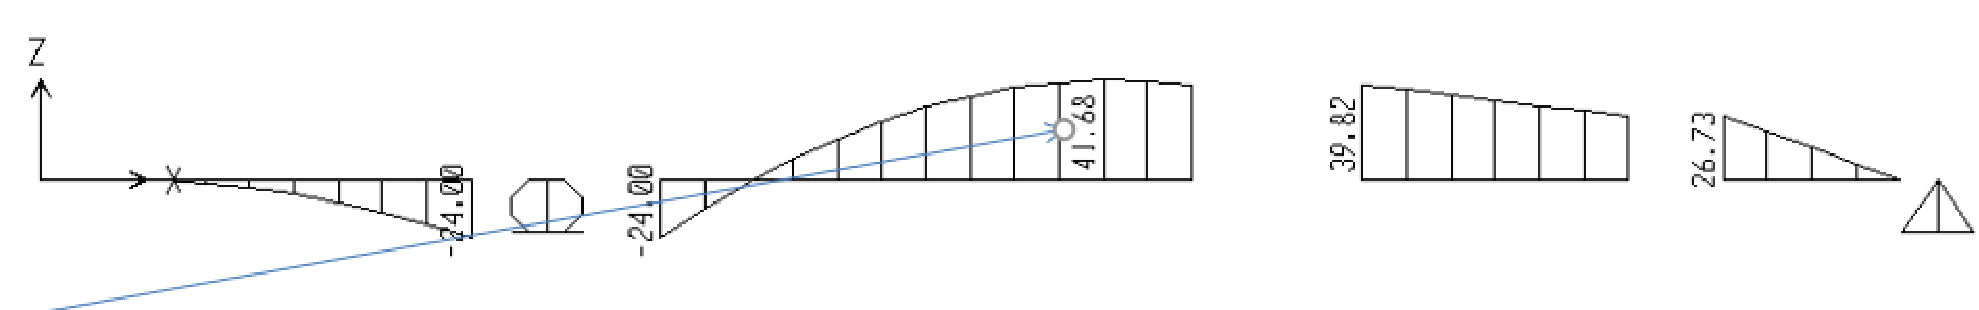
\includegraphics[width=0.5\textwidth]{mm45.pdf}
  \caption{Diagrama de momentos en SAP2000}
  \label{mm45}
\end{figure}
Resultando de la tabla generada un momento máximo de 41.536 y de forma precisa está en x=5.12 y $M_{max}=41.72$, se usará éste momento para diseñar.

\begin{example}
    Proponiendo una sección diferente, nótese que en la figura \ref{mm46} el elemento 1 de 20cm por 2.65cm, la sección dos de (48.85 por 1cm) y la  sección tres con base de 40 y altura de 15
\end{example}

\textit{ Sol. }

Calculando el centroide, se calcula el área de cada una, luego de los datos de la tabla \ref{tabmm10}
\begin{table}[h!]
    \centering
    \begin{tabular}{@{}lccclll@{}}
    \toprule
                         & AREA   & yi     & A(yi)      & \multicolumn{1}{c}{d} & \multicolumn{1}{c}{$A(d_2)$}   & \multicolumn{1}{c}{$Ip$} \\ \midrule
    1                    & 53     & 48.675 & 2579.775   & 25.1014322            & 33394.3405                     & 31.0160417               \\
    2                    & 45.85  & 24.425 & 1119.88625 & 0.85143217            & 33.2383494                     & 8032.2418                \\
    3                    & 60     & 0.75   & 45         & -22.8235678           & 31254.9149                     & 11.25                    \\
    \multicolumn{1}{c}{} & 158.85 &        & 3744.66125 & \multicolumn{1}{c}{}  & \multicolumn{1}{c}{64682.4938} & 8074.50784               \\ \bottomrule
    \end{tabular}
    \caption{Cálculos iniciales para el cálculo del centroide de una viga}
    \label{tabmm10}
\end{table}
Recordando que $Y_C=\frac{\sum A(y_i)}{\sum A}$ encontrando que el centroide $y_c=23.57$cm, es decir que la vertical $c_y=23.57$ y del centroide hacia el elemento 1=26.42cm.
Para calcular el momento debe ser $I=\sum\left(I_p\right)+\sum Ad^2$, desarrollando los cálculos:
\begin{align*}
    &I =72757.002cm^4&&y 26.4264cm&&M_{max} =4172231.4kg\cdot cm\\
    &esf=1515.4169\frac{kg}{cm^2}&&f_y=2530kg^2/cm&&f_{\max}= 1518 \frac{kg}{cm^2}\\
    &f_{\max} =1518 \frac{kg}{cm^2}&&E = 2 \times 10^7 ton/m^2&&6EI = 8.7 \times 1^{4}\\
    &Des= 0.018m&&Des 187798cm&&
\end{align*}

\begin{example}
  De la viga que tiene dos apoyos, se nota que las 12 Toneladas es $2T/m\cdot 6m$, equilibrado con las fuerzas inferiores verticales (6 y 6 Ton), pensando en un problema que tenga tres apoyos como en la figura \ref{mm}
\begin{figure}[h!]
\centering
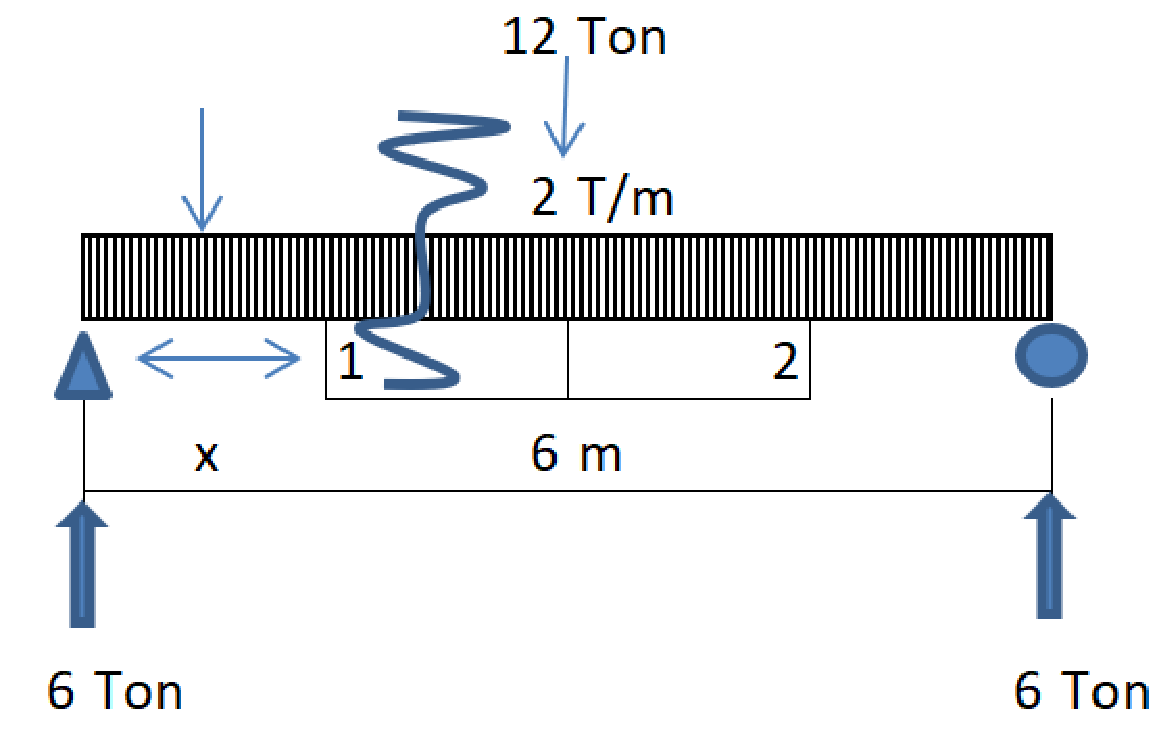
\includegraphics[width=0.5\textwidth]{mm46.pdf}
\caption{Esquema del problema}
\label{mm46}
\end{figure}
\end{example}
\textit{ Sol. }
Existen diferentes formas de resolverlo, primero quitando el apoyo (lo que se hizo anteriormente), y se va a calcular el desplazamiento que ocurrió en el centro del plano a tres metros del apoyo como en la tabla \ref{tabmm11}
\begin{table}[h!]\centering
  \begin{tabular}{@{}ccccc@{}}
  \toprule
  inte & M     & m    & int(Mm) &       \\ \midrule
  3    & 0     & 0    & 0       &       \\
  1    & 12    & 6.75 & 0.75    & 60.75 \\
  3    & 9     & 1.5  & 40.5    &       \\
  3    & 9     & 1.5  & 40.5    &       \\
  2    & 12    & 6.75 & 0.75    & 60.75 \\
  3    & 0     & 0    & 0       &       \\
  suma & 202.5 &      &         &       \\ \bottomrule
  \end{tabular}
  \caption{Cálculo del desplazamiento}
  \label{tabmm111}
\end{table}
El valor suma de 202.5 debe dividirse entre $EI$, en cuanto sea constante no habría problema.

Ahora el desplazamiento generado en la viga con una \textbf{carga unitaria} como se nota en la figura \ref{mm47}
\begin{figure}[h!]
\centering
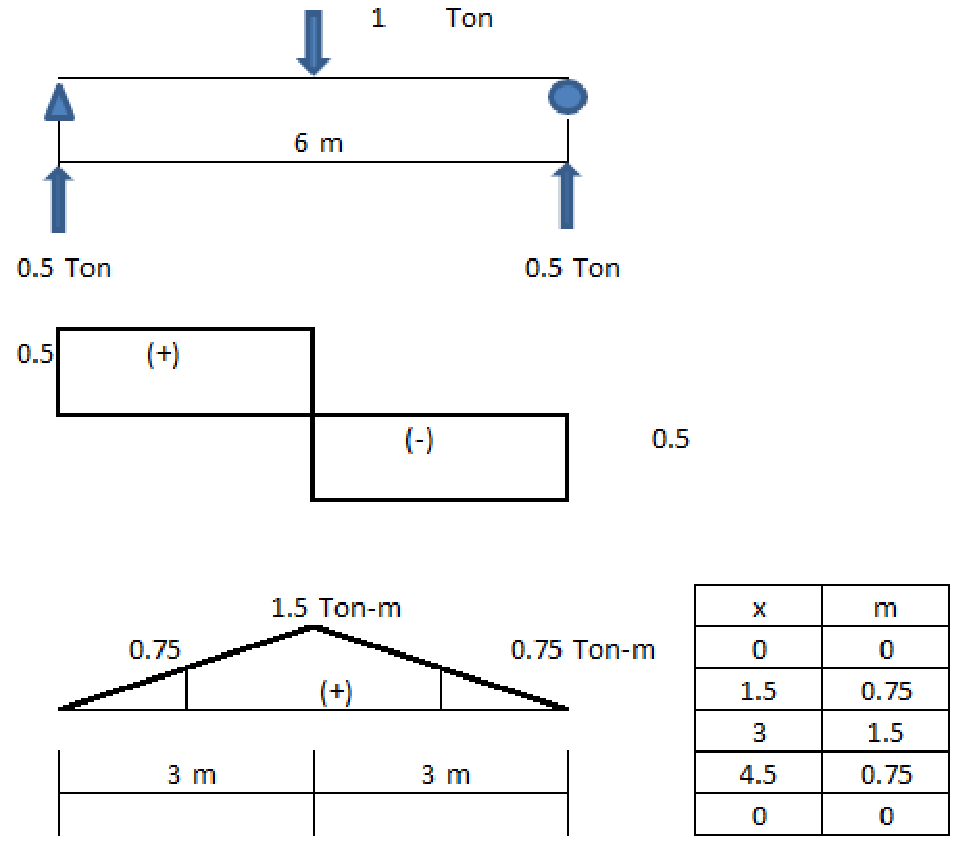
\includegraphics[width=0.5\textwidth]{mm47.pdf}
\caption{Desplazamiento de la viga}
\label{mm47}
\end{figure}
Se tiene que RC=7.5 Ton la cual es la fuerza que debe ser colocada en el centro para encontrar el equilibrio.
Trasladandolo a un problema más complejo, se dividirá entre los dos apoyos porque son simétricos, la suma de los tres apoyos debe ser 12 Ton. Analíce la siguiente gráfica:
\begin{figure}[h!]
\centering
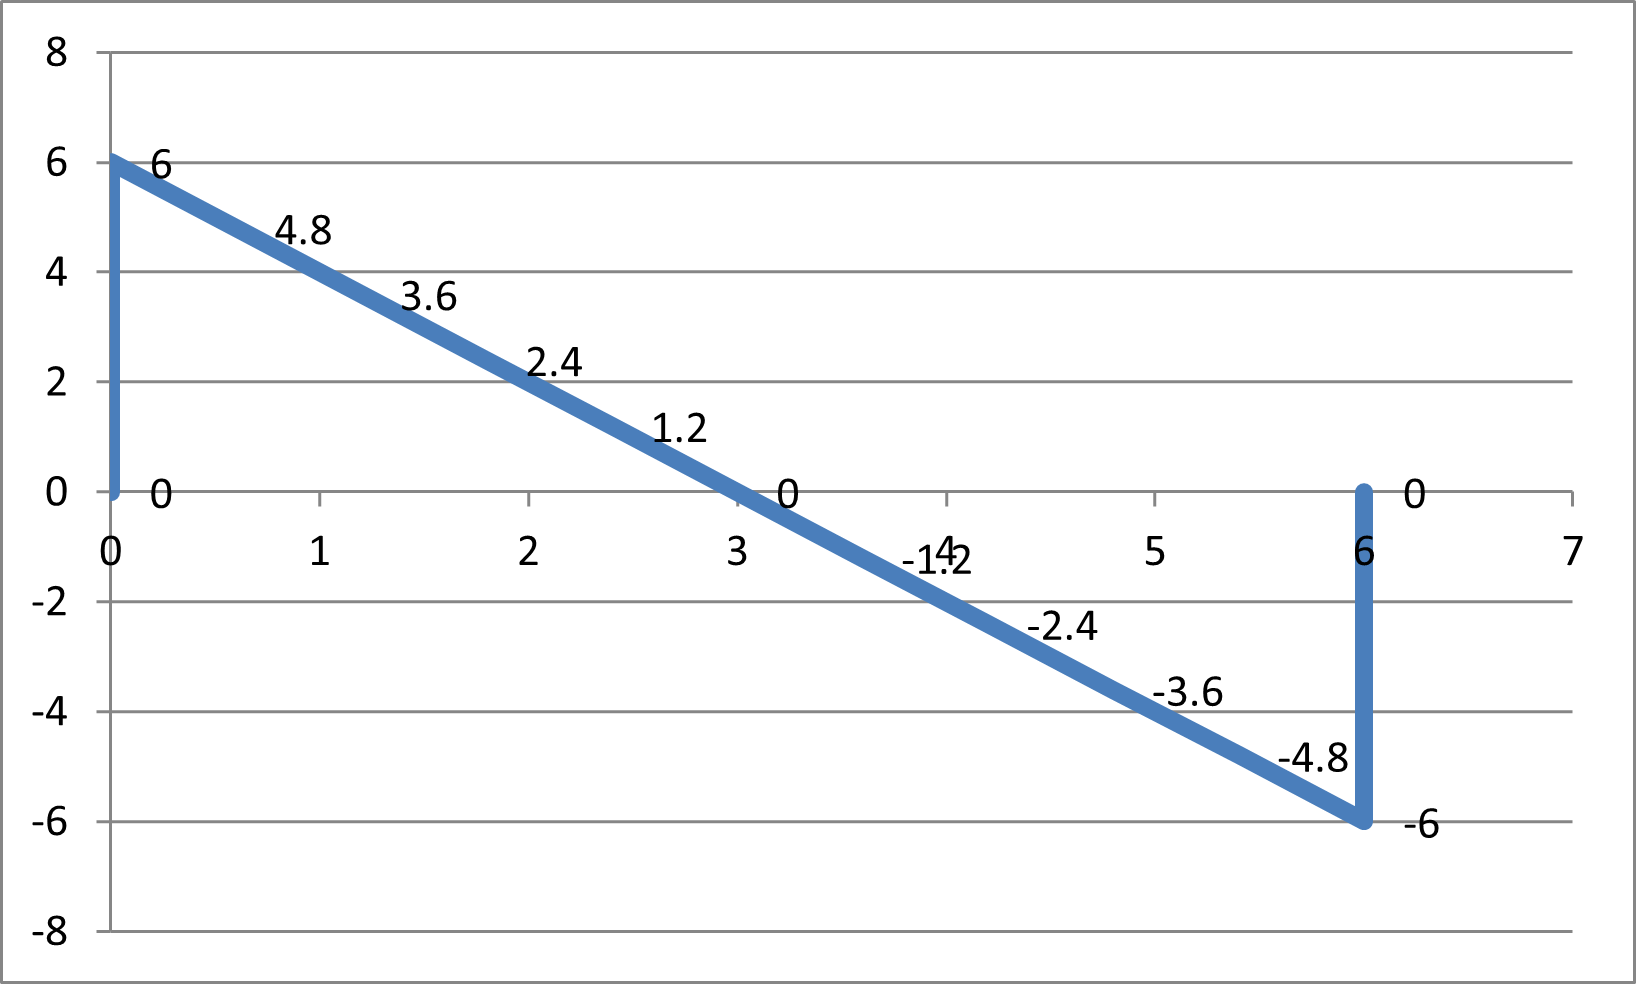
\includegraphics[width=0.5\textwidth]{mm49.png}
\caption{Diagrama de cortantes}
\label{mm49}
\end{figure}
Calculando la ecuación de momento, obtenemos una gráfica así:
\begin{figure}[h!]
\centering
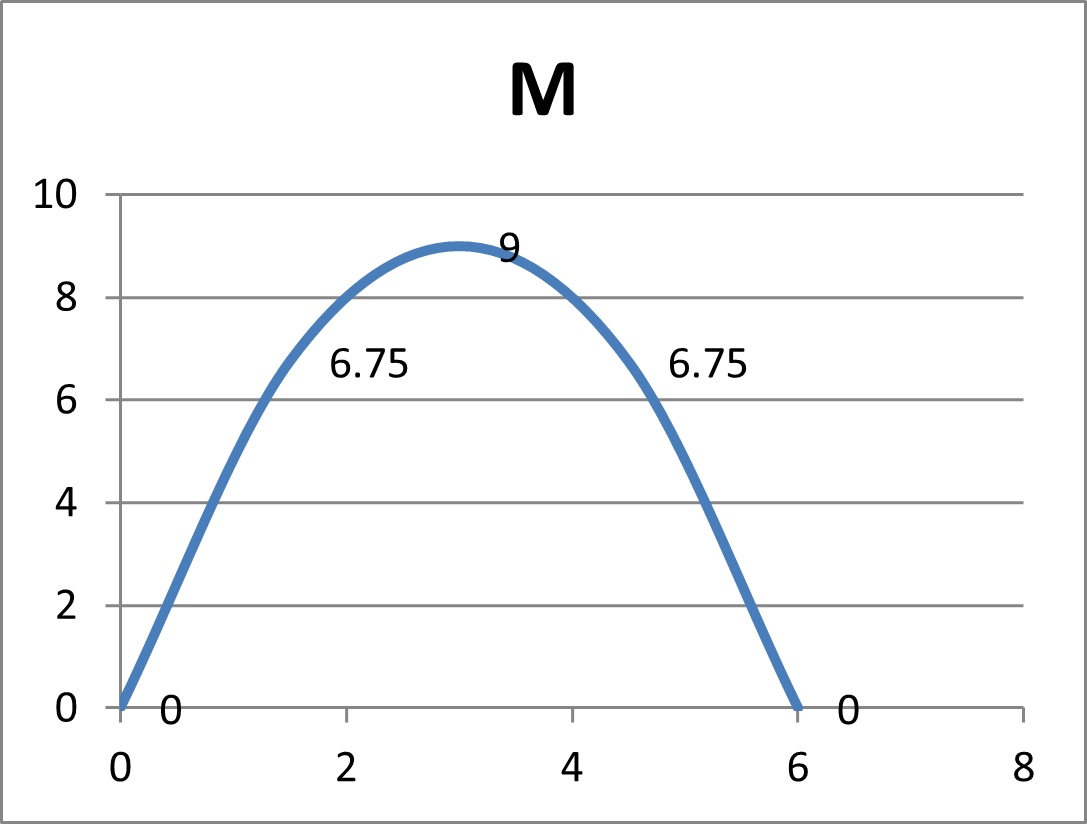
\includegraphics[width=0.5\textwidth]{mm50.png}
\caption{Diagrama de momentos}
\label{mm50}
\end{figure}
%%
%
%
%
%
%
%%
%
%
Del esquema \ref{mm51}, se resuelve la viga isostática.
\begin{figure}[h!]
\centering
  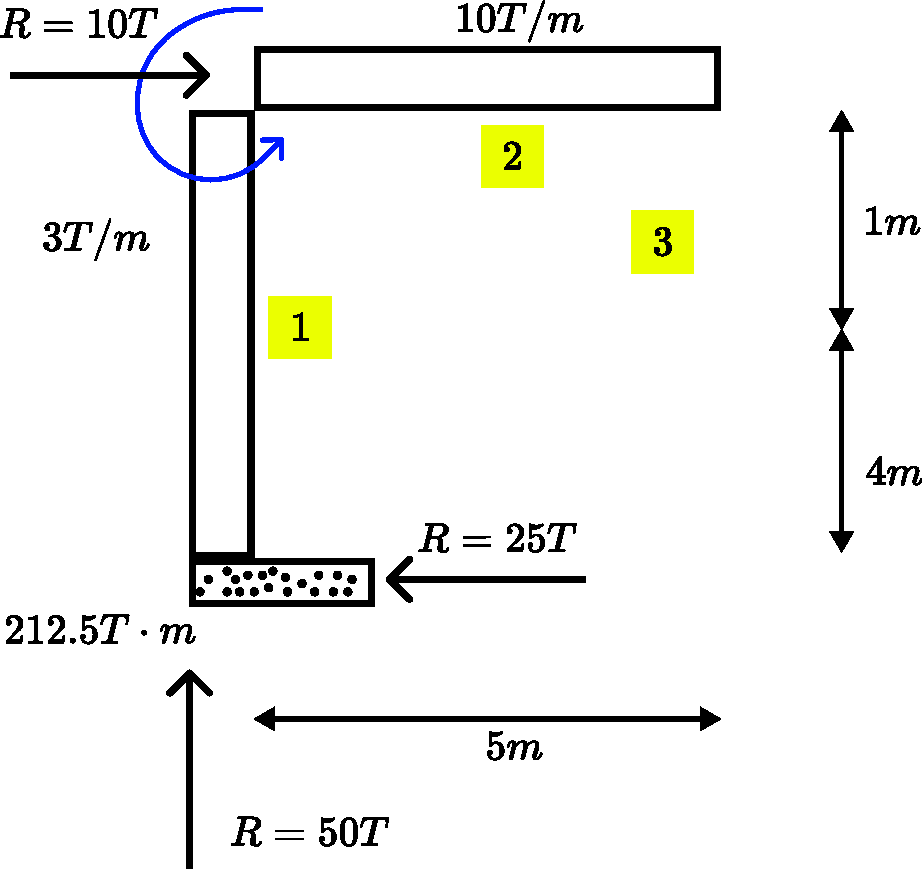
\includegraphics[width=0.5\textwidth]{mm51.pdf}
  \caption{Esquema del problema}
  \label{mm51}
\end{figure}
Se obtienen los valores de los momentos al inicio, en medio y al final de la barrera en la figura \ref{2}.

\begin{figure}[h!]
\centering
  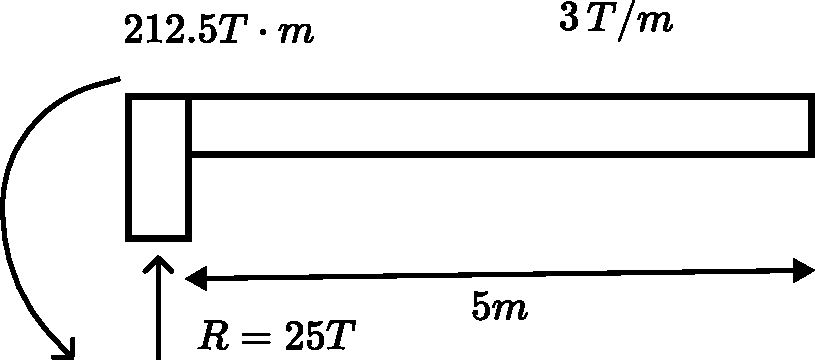
\includegraphics[width=0.5\textwidth]{mm52.pdf}
  \caption{Análisis de momentos}
  \label{mm52}
\end{figure}
del cual desarrollamos:
\begin{align*}
    &V=25-3x\\
    &M=25x-\frac{3}{2}x^2-212.5
\end{align*}
Del cual los momentos son:
\begin{table}[h!]
\centering
\begin{tabular}{@{}cc@{}}
\toprule
x   & m      \\ \midrule
0   & 0      \\
2.5 & 159.37 \\
5   & 125    \\ \bottomrule
\end{tabular}
\caption{Momentos}
\label{tabmm12}
\end{table}
Para la sección 2:
\begin{figure}[h!]
\centering
  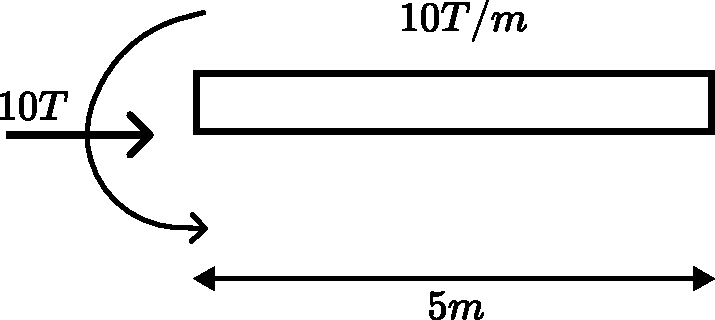
\includegraphics[width=0.5\textwidth]{mm53.pdf}
  \caption{a}
  \label{mm533}
\end{figure}
De manera que $V=50-10x$ y esto implica que:
\begin{equation}
    M=50x-\frac{10}{2}x^2-125
\end{equation}
Obteniendo las $M$ y $V$:
\begin{table}[ht!]
\centering
\begin{tabular}{@{}ccc@{}}
\toprule
x   & V  & M      \\ \midrule
0   & 50 & -125   \\
2.5 & 25 & -31.25 \\
5   & 0  & 0      \\ \bottomrule
\end{tabular}
\caption{Cortantes y Momentos para la sección 2}
\label{tabmm13}
\end{table}
Para la tercera sección, no se cuenta con cargas pero sus momentos son iguales a cero, por lo tanto concentramos la información se las tablas \ref{tab1} y \ref{tab2} se obtiene la tabla \ref{tab3}
\begin{table}[h!]
\centering
\begin{tabular}{@{}cc@{}}
\toprule
Sección            & p       \\ \midrule
\multirow{3}{*}{1} & -121    \\
                   & -159.38 \\
                   & -125    \\
\multirow{3}{*}{2} & -125    \\
                   & -31.25  \\
                   & 0       \\
\multirow{3}{*}{3} & 0       \\
                   & 0       \\
                   & 0       \\ \cmidrule(l){2-2} 
\end{tabular}
\caption{P totales}
\label{tab3}
\end{table}
Procedemos a quitar el apoyo que se pone al final de la barra tres para colocar una fuerza unitaria. Recordando que el momento es $F\cdot d=\mu$ se obtiene $m$; con la integral se obtiene la reacción para la estructura hiperestática, se puede  hacer un problema para un empotramiento en la parte inferior de la viga tres empleando matrices, por lo que para diseñar la columna de acero (Hiperestática) se requiere que la fuerza produzca un esfuerzo carga entre área y el momento máximo:
\begin{equation}
    \sigma=\frac{Cort_{\max}}{Área_{alma}}
\end{equation}
También se hace un análisis para diseñar la viga (Concreto), se revisa la cantidad de acero, tanto varillas como estribos.





